\renewcommand*\chappic{img/diff-crypt.pdf}
\renewcommand*\chapquote{Just because it's automatic doesn't mean it works.}
\renewcommand*\chapquotesrc{Daniel J. Bernstein}
%
\chapter{Differential cryptanalysis}
\label{ch:dc}
%
In Chapter~\ref{ch:hash} we defined two hash functions. In this chapter
we consider such functions from a differential perspective. Differential
cryptanalysis will turn out to yield successful collision attacks on hash
functions. We introduce a notation to easily represent differential
characteristics.

\section{Motivation}
\label{sec:dc-motivation}
%
In August 2004, Wang et al. published results at Crypto'04~\cite{wang2004} which revealed
that MD4, MD5, HAVAL-128 and RIPEMD can be broken practically using differential cryptanalysis.
Their work is based on preliminary work by Hans Dobbertin~\cite{Dobbertin1998}.
On an IBM~P690 machine, an MD5 collision can be computed in about one hour using this approach.
Collisions for HAVAL-128, MD4 and RIPEMD were found as well. Patrick Stach's \texttt{md4coll.c}
program~\cite{md4coll} implements Wang's approach and can find MD4 collisions in few seconds
on my Thinkpad~x220 setup specified in Appendix~\ref{app:setup}.

Let $n$ denote the digest size, i.e. the size of the hash value $h(x)$ in bits.
Due to the birthday paradox, a collision attack has a generic complexity of $2^{n/2}$
whereas preimage and second preimage attacks have generic complexities of $2^n$.
In other words it is computationally easier to find any two colliding hash values
than the preimage or second preimage for a given hash value.

Following results by Wang et al., differential cryptanalysis was shown as
powerful tool for cryptanalysis of hash algorithms. This thesis applies those
ideas to satisfiability approaches.

\begin{table}[bt]
  \begin{center}
    \begin{tabular}{cccc}
      \hline \hline
      \multicolumn{4}{c}{Message 1} \\
      \hline
        4d7a9c83 & \textbf{d6cb927a} & \textbf{29d5a578} & 57a7a5ee \\
        de748a3c & dcc366b3 & b683a020 & 3b2a5d9f \\
        c69d71b3 & f9e99198 & d79f805e & a63bb2e8 \\
        \textbf{45dc8e31} & 97e31fe5 & 2794bf08 & b9e8c3e9 \\
      \hline
      \multicolumn{4}{c}{Message 2} \\
      \hline
        4d7a9c83 & \textbf{56cb927a} & \textbf{b9d5a578} & 57a7a5ee \\
        de748a3c & dcc366b3 & b683a020 & 3b2a5d9f \\
        c69d71b3 & f9e99198 & d79f805e & a63bb2e8 \\
        \textbf{45dd8e31} & 97e31fe5 & 2794bf08 & b9e8c3e9 \\
      \hline
      \multicolumn{4}{c}{Hash value of Message 1 and Message 2} \\
      \hline
        5f5c1a0d & 71b36046 & 1b5435da & 9b0d807a \\
      \hline \hline
    \end{tabular}
    \caption[Hexadecimal values of one MD4 collisions given in paper~\cite{wang2004}]{
      One of two MD4 hash collisions provided in~\cite{wang2004}.
      A message represents one block of 512~bits.
      %The hash value consists of 128~bits.
      Values are given in hexadecimal, message words are enumerated from
      left to right, top to bottom. Differences are highlighted in
      bold for illustration purposes. For comparison the first bits
      of Message 1 are \texttt{11000001\dots} and the last bits are
      \texttt{\dots10011101}.
    }
    \label{tab:wang-md4-collision1}
  \end{center}
\end{table}

\newpage
\section{Fundamentals}
\label{sec:dc-fundamentals}
%
\index{Hash collision}
\begin{defi}[Hash collision]
  Given a hash function $h$,
  a hash collision is a pair $(x_1, x_2)$ with $x_1 \neq x_2$ such that
  $h(x_1) = h(x_2)$.
\end{defi}

\index{Pseudo-collision}
Pseudo-collisions are also often considered when attacking hash functions.
A \emph{pseudo-collision} is given if a hash collision can be found for a given
hash function, but the initial vectors (IV) can be chosen for each message.

Hash algorithms consume input values as blocks of bits.
As far as the length of the input must not conform to the block size,
padding is applied. Now consider such a block of input values
and another copy of it. We use those two blocks as inputs for two
hash algorithm instances, but provide slight modifications in few bits.
Differential cryptanalysis is based on the idea to consider those execution states
and trace those differences to learn about the propagation of message differences.
Compare this setup with Figure~\ref{tab:collision-attack}.

\index{Avalanche effect}
At the very beginning only the few defined differences are given. But as the
hash algorithm progresses in computation, differences are propagated to more
and more bits. Most likely the final value will differ in many bits, because
of a desirable hash algorithm property called \emph{avalanche effect}.
A small difference in the input should lead to a significant difference
in the output (i.e. visually recognizable).

Visualizing those differences helps the cryptanalyst to find modifications
yielding a small number of differences in the evaluation state. Empirical
results in differential cryptanalysis indicate that sparse characteristics
are desirable, because it is easier to cancel out few differences in the
output compared to many differences.
The cryptanalyst consecutively modifies the input values to eventually
receive a collision in the output value (i.e. $\Delta C = 0 \iff C = C^*$).

\index{Differential path}
\index{Differential characteristic}
\begin{defi}
  The differential state during a computation is called
  \emph{differential characteristic} (also \emph{differential path}).
\end{defi}

\begin{theorem}
  Assuming the number of differences in a differential characteristic is small,
  this characteristic is expected to result in a hash collision with higher probability.
\end{theorem}

\begin{figure}[bt]
  \begin{center}
    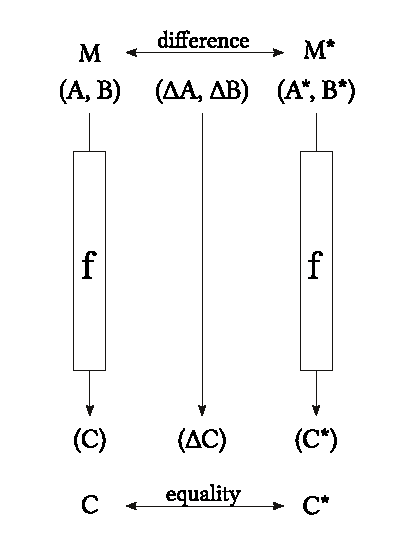
\includegraphics[width=0.55\textwidth]{img/diff_cryptanalysis.pdf}
    \caption[Common attack setting for a collision attack]{
      Common attack setting for a collision attack:
      Hash function $f$ is applied to two inputs $M$ and $M^*$ which differ
      by some predefined bits. $\Delta M$ describes the difference between
      these values. A hash collision is given if and only if output values
      $C$ and $C^*$ show the same value. In differential cryptanalysis we observe
      the differences between two instances applying function $f$
      to inputs $M$ and $M^*$.
    }
    \label{tab:collision-attack}
  \end{center}
\end{figure}

\section{Differential notation}
\label{sec:dc-notation}
%
\index{Bit condition}
\index{Generalized bit condition}
\index{Differential notation}
Differential notation helps us to visualize differential characteristics
by defining so-called \emph{generalized bit conditions}.
It was introduced by Christophe de Canni\`ere and Christian Rechberger
in 2006~\cite[Section 3.2]{char-2006}, inspired by \emph{signed differences} by
Wang~et al. and is shown in Table~\ref{tab:diff-notation}.

\begin{table}[!ht]
  \small
  \begin{center}
    \begin{tabular}{|c|cccc|}
    \hline\hline
      $(x_i, x_i^*)$ & $(0,0)$ & $(1,0)$ & $(0,1)$ & $(1,1)$ \\
    \hline
      \dnI{?}        & \yes    & \yes    & \yes    & \yes    \\
      \dnI{-}        & \yes    & \no     & \no     & \yes    \\
      \dnI{x}        & \no     & \yes    & \yes    & \no     \\
      \dnI{0}        & \yes    & \no     & \no     & \no     \\
      \dnI{u}        & \no     & \yes    & \no     & \no     \\
      \dnI{n}        & \no     & \no     & \yes    & \no     \\
      \dnI{1}        & \no     & \no     & \no     & \yes    \\
      \dnI{\#}       & \no     & \no     & \no     & \no     \\
    \hline \hline
    \end{tabular}
    \begin{tabular}{|c|cccc|}
    \hline\hline
      $(x_i, x_i^*)$ & $(0,0)$ & $(1,0)$ & $(0,1)$ & $(1,1)$ \\
    \hline
      \dnI{3}        & \yes    & \yes    & \no     & \no     \\
      \dnI{5}        & \yes    & \no     & \yes    & \no     \\
      \dnI{7}        & \yes    & \yes    & \yes    & \no     \\
      \dnI{A}        & \no     & \yes    & \no     & \yes    \\
      \dnI{B}        & \yes    & \yes    & \no     & \yes    \\
      \dnI{C}        & \no     & \no     & \yes    & \yes    \\
      \dnI{D}        & \yes    & \no     & \yes    & \yes    \\
      \dnI{E}        & \no     & \yes    & \yes    & \yes    \\
    \hline \hline
    \end{tabular}
    \caption[Differential notation as introduced in~\cite{char-2006}]{
      Differential notation as introduced in~\cite{char-2006}.
      The left-most column specifies a symbol called \enquote{bit condition}
      and right-side columns indicate which bit configurations
      are possible for two given bits $x_i$ and $x_i^*$.
    }
    \label{tab:diff-notation}
  \end{center}
\end{table}

Consider two hash algorithm instances. Let $x_i$ be some bit
from the first instance and let $x_i^*$ be the corresponding bit
from the second instance. Differences are computed using a \boolf{XOR}
and commonly denoted as $\Delta x = x_i \oplus x_i^*$.
Bit conditions allow us to encode possible relations between bits $x_i$ and $x_i^*$.

For example, let us take a look at the original Wang et al. hash collision
in MD4 provided in Table~\ref{tab:wang-md4-collision1}.
We extract all values with differences and represent them using differential notation.
This gives us Table~\ref{tab:differential-wang-values}.

\begin{table}[!ht]
  \begin{center}
    \small
    \begin{tabular}{ccl}
      \hline \hline
      bit & hexadecimal & binary representation / differential notation \\
      \hline \hline
      $x_0$ & \dnI{d6cb927a} & \dnI{11010110110010111001001001111010} \\
      $x_1$ & \dnI{29d5a578} & \dnI{00101001110101011010010101111000} \\
      $x_2$ & \dnI{45dc8e31} & \dnI{01000101110111001000111000110001} \\
      \hline
      $x_0^*$ & \dnI{56cb927a} & \dnI{01010110110010111001001001111010} \\
      $x_1^*$ & \dnI{b9d5a578} & \dnI{10111001110101011010010101111000} \\
      $x_2^*$ & \dnI{45dd8e31} & \dnI{01000101110111011000111000110001} \\
      \hline
      $\Delta x$ & & \dnI{u1010110110010111001001001111010} \\
                 & & \dnI{n01n1001110101011010010101111000} \\
                 & & \dnI{010001011101110n1000111000110001} \\
      \hline \hline
    \end{tabular}
    \caption[Bit differences in the original Wang et al. hash collision]{
      The three words different between Message~1 and Message~2 of the original
      MD4 hash collision by Wang et al. The last three lines show
      how differences can be
      written down using bit conditions. As far as 4 symbols are not from the
      set $\set{0, 1}$ it holds that the messages differ by 4~bits.
    }
    \label{tab:differential-wang-values}
  \end{center}
\end{table}

The following properties hold for bit conditions:
\begin{itemize}[noitemsep,topsep=0pt]
  \item If $x_i = x_i^*$ holds and some value is known, $\set{0,1}$ contains its bit condition.
  \item If $x_i \neq x_i^*$ holds and some value is known, $\set{u,n}$ contains its bit condition.
  \item If $x_i = x_i^*$ holds and the values are unknown, its bit condition is $\dnI{-}$.
  \item If $x_i \neq x_i^*$ holds and the values are unknown, its bit condition is $\dnI{x}$.
\end{itemize}
Applying this notation to hash collisions means that arbitrary bit conditions
(except for \dnI{\#}) can be specified for the input values. In one of the
intermediate iterations, we enforce a difference using one of the bit conditions
$\set{u,n,x}$. This excludes trivial solutions with no differences from the set of
possible solutions. And the final values need to lack differences thus are
represented using a dash \dnI{-}.

\begin{table}[!ht]
  \begin{center}
    \begin{tabular}{cp{5cm}cl}
      $\Delta x$      & conjunctive normal form &
      $\Delta x$      & conjunctive normal form \\
    \hline
      \dnI{\#}        & $(x) \land (\neg x)$ &
      \dnI{1}         & $(x) \land (x^*)$ \\

      \dnI{0}         & $(\neg x) \land (\neg x^*)$ &
      \dnI{-}         & $\neg (x \oplus x^*)$ \\

      \dnI{u}         & $(x) \land (\neg x^*)$ &
      \dnI{A}         & $(x)$ \\

      \dnI{3}         & $(\neg x^*)$ &
      \dnI{B}         & $(x \lor \neg x^*)$ \\

      \dnI{n}         & $(\neg x) \land (x^*)$ &
      \dnI{C}         & $(x^*)$ \\

      \dnI{5}         & $(\neg x)$ &
      \dnI{D}         & $(\neg x \lor x^*)$ \\

      \dnI{x}         & $(x \oplus x^*)$ &
      \dnI{E}         & $(x \lor x^*)$ \\

      \dnI{7}         & $(\neg x \lor \neg x^*)$ &
      \dnI{?}         &  \\
    \end{tabular}
    \caption[Representation of bit conditions as CNF]{%
      All bit conditions represented as CNF using
      two Boolean variables $x$ and $x^*$ to represent
      two bits.
    }
    \label{tab:simple-eval-clauses}
  \end{center}
\end{table}


\section{A simple addition example}
\label{sec:dc-example}
%
Using this notation, we can now reason about the behavior of functions on differential values.
We start with 1-bit addition as basic exercise to the reader. Consider a matrix with
two input rows and one output row. The values of the first two rows are added such that
the bit difference at the third row is created.

\begin{figure}[!ht]
  \begin{center}
    \begin{minipage}{20pt}\begin{tabular}{c} \dnI{-} \\ \dnI{-} \\ \hline \dnI{-} \end{tabular}\end{minipage}
    \hspace{20pt}$\Rightarrow$\hspace{20pt}
    \begin{minipage}{20pt}\begin{tabular}{c} \dnI{0}\dnI{0} \\ \dnI{0}\dnI{0} \\ \hline \dnI{0}\dnI{0} \end{tabular}\end{minipage}
    \begin{minipage}{20pt}\begin{tabular}{c} \dnI{0}\dnI{0} \\ \dnI{0}\dnI{0} \\ \hline \dnI{1}\dnI{1} \end{tabular}\end{minipage}
    \begin{minipage}{20pt}\begin{tabular}{c} \dnI{0}\dnI{0} \\ \dnI{1}\dnI{1} \\ \hline \dnI{0}\dnI{0} \end{tabular}\end{minipage}
    \begin{minipage}{20pt}\begin{tabular}{c} \dnI{0}\dnI{0} \\ \dnI{1}\dnI{1} \\ \hline \dnI{1}\dnI{1} \end{tabular}\end{minipage}
    \begin{minipage}{20pt}\begin{tabular}{c} \dnI{1}\dnI{1} \\ \dnI{0}\dnI{0} \\ \hline \dnI{0}\dnI{0} \end{tabular}\end{minipage}
    \begin{minipage}{20pt}\begin{tabular}{c} \dnI{1}\dnI{1} \\ \dnI{0}\dnI{0} \\ \hline \dnI{1}\dnI{1} \end{tabular}\end{minipage}
    \begin{minipage}{20pt}\begin{tabular}{c} \dnI{1}\dnI{1} \\ \dnI{1}\dnI{1} \\ \hline \dnI{0}\dnI{0} \end{tabular}\end{minipage}
    \begin{minipage}{20pt}\begin{tabular}{c} \dnI{1}\dnI{1} \\ \dnI{1}\dnI{1} \\ \hline \dnI{1}\dnI{1} \end{tabular}\end{minipage}
    \caption[A simple 1-bit addition example]{%
      A simple 1-bit addition example:
      On the left the differential characteristic is given.
      Two dashes, by definition, denote a missing difference in both arguments.
      The result of the addition must never show a difference.
      This yields eight possible bit configurations where two values close to each other denote $(M, M^*)$ of Figure~\ref{tab:collision-attack}.
      Due to the behavior of addition, we know that configurations 2, 3, 5 and 8 (from left to right) are invalid.
    }
    \label{fig:1-bit-example}
  \end{center}
\end{figure}

Figure~\ref{fig:1-bit-example} illustrates this example. Remember that symbols such as
\dnI{-} and \dnI{0} underlie semantics defined in Table~\ref{tab:diff-notation}.
It is also interesting to see how propagation of values can work. In
Figure~\ref{fig:1-bit-deduction} we see how an underspecified value \dnI{?} can be
strengthened once we have checked which values can be taken. Recognize that the
system is constrained by the function in use and the definition of the differential symbols.

\begin{figure}[!ht]
  \begin{center}
    \begin{minipage}{20pt}\begin{tabular}{c} \dnI{-} \\ \dnI{-} \\ \hline \dnI{?} \end{tabular}\end{minipage}
    \hspace{20pt}$\Rightarrow$\hspace{20pt}
    \begin{minipage}{20pt}\begin{tabular}{c} \dnI{0}\dnI{0} \\ \dnI{0}\dnI{0} \\ \hline \dnI{0}\dnI{0} \end{tabular}\end{minipage}
    \begin{minipage}{20pt}\begin{tabular}{c} \dnI{0}\dnI{0} \\ \dnI{1}\dnI{1} \\ \hline \dnI{1}\dnI{1} \end{tabular}\end{minipage}
    \begin{minipage}{20pt}\begin{tabular}{c} \dnI{1}\dnI{1} \\ \dnI{0}\dnI{0} \\ \hline \dnI{1}\dnI{1} \end{tabular}\end{minipage}
    \begin{minipage}{20pt}\begin{tabular}{c} \dnI{1}\dnI{1} \\ \dnI{1}\dnI{1} \\ \hline \dnI{0}\dnI{0} \end{tabular}\end{minipage}
    \caption[Propagation of bit conditions in a differential characteristic]{%
      Like Figure~\ref{fig:1-bit-example}, but any difference value for the result bit is possible.
      As such we consider any possible bit configuration, but eventually recognize that only four bit configurations
      are consistent with the behavior of addition. Because all resulting configurations show no bit difference
      in the output bit, we can strengthen \dnI{?} by replacing it with \dnI{-}. This illustrates how
      knowledge about differential states can be propagated.
    }
    \label{fig:1-bit-deduction}
  \end{center}
\end{figure}

Finally, we can extend our testcases to 4~bits and retrieve testcases such as
Figures~\ref{fig:4-bit-addition} and \ref{fig:sigma}.

\begin{figure}[!ht]
  \begin{center}
    \begin{minipage}{0.23\textwidth}
      \begin{tabular}{rl}
        A: & \dnI{0}\dnI{0}\dnI{1}\dnI{1} \\
        B: & \dnI{0}\dnI{1}\dnI{0}\dnI{1} \\
        S: & \dnI{1}\dnI{0}\dnI{0}\dnI{0}
      \end{tabular}
    \end{minipage}
    \begin{minipage}{0.23\textwidth}
      \begin{tabular}{rl}
        A: & \dnI{-}\dnI{-}\dnI{-}\dnI{x} \\
        B: & \dnI{-}\dnI{-}\dnI{-}\dnI{x} \\
        S: & \dnI{?}\dnI{?}\dnI{?}\dnI{?}
      \end{tabular}
    \end{minipage}
    \begin{minipage}{0.23\textwidth}
      \begin{tabular}{rl}
        A: & \dnI{-}\dnI{-}\dnI{-}\dnI{x} \\
        B: & \dnI{-}\dnI{-}\dnI{-}\dnI{x} \\
        S: & \dnI{?}\dnI{?}\dnI{?}\dnI{-}
      \end{tabular}
    \end{minipage}
    \begin{minipage}{0.23\textwidth}
      \begin{tabular}{rl}
        A: & \dnI{-}\dnI{-}\dnI{-}\dnI{x} \\
        B: & \dnI{-}\dnI{-}\dnI{-}\dnI{x} \\
        S: & \dnI{x}\dnI{?}\dnI{?}\dnI{?}
      \end{tabular}
    \end{minipage}
  \end{center}%

  \begin{center}
    \begin{minipage}{0.23\textwidth}
      \begin{tabular}{rl}
        A: & \dnI{0}\dnI{0}\dnI{1}\dnI{1} \\
        B: & \dnI{0}\dnI{1}\dnI{0}\dnI{1} \\
        S: & \dnI{0}\dnI{0}\dnI{0}\dnI{0}
      \end{tabular}
    \end{minipage}
    \begin{minipage}{0.23\textwidth}
      \begin{tabular}{rl}
        A: & \dnI{-}\dnI{-}\dnI{-}\dnI{x} \\
        B: & \dnI{-}\dnI{-}\dnI{-}\dnI{x} \\
        S: & \dnI{?}\dnI{?}\dnI{?}\dnI{x}
      \end{tabular}
    \end{minipage}
    \begin{minipage}{0.23\textwidth}
      \begin{tabular}{rl}
        A: & \dnI{-}\dnI{-}\dnI{-}\dnI{-} \\
        B: & \dnI{-}\dnI{-}\dnI{-}\dnI{x} \\
        S: & \dnI{x}\dnI{-}\dnI{?}\dnI{?}
      \end{tabular}
    \end{minipage}
  \end{center}%
  \caption[
    Testcases for 4-bit addition
  ]{
    Testcases for 4-bit addition:
    The upper line shows valid differential characteristics for 4-bit addition
    whereas the lower line show invalid ones for 4-bit addition.
    The rows are conventionally named using capital letters.
  }
  \label{fig:4-bit-addition}
\end{figure}

\begin{figure}[!ht]
  \begin{center}
    \begin{minipage}{0.23\textwidth}
      \begin{tabular}{rl}
        A: & \dnI{-}\dnI{-}\dnI{-}\dnI{-} \\
        S: & \dnI{0}\dnI{0}\dnI{0}\dnI{0}
      \end{tabular}
    \end{minipage}
    \begin{minipage}{0.23\textwidth}
      \begin{tabular}{rl}
        A: & \dnI{7}\dnI{C}\dnI{-}\dnI{3} \\
        S: & \dnI{-}\dnI{3}\dnI{u}\dnI{?}
      \end{tabular}
    \end{minipage}
    \begin{minipage}{0.23\textwidth}
      \begin{tabular}{rl}
        A: & \dnI{0}\dnI{u}\dnI{C}\dnI{D} \\
        S: & \dnI{A}\dnI{D}\dnI{C}\dnI{7} \\
      \end{tabular}
    \end{minipage}
  \end{center}

  \begin{center}
    \begin{minipage}{0.23\textwidth}
      \begin{tabular}{rl}
        A: & \dnI{-}\dnI{-}\dnI{-}\dnI{x} \\
        S: & \dnI{0}\dnI{0}\dnI{0}\dnI{0}
      \end{tabular}
    \end{minipage}
    \begin{minipage}{0.23\textwidth}
      \begin{tabular}{rl}
        A: & \dnI{x}\dnI{x}\dnI{x}\dnI{x} \\
        S: & \dnI{0}\dnI{0}\dnI{0}\dnI{0} \\
      \end{tabular}
    \end{minipage}
  \end{center}
  \caption[Differential characteristics for the SHA-2 Sigma function]{
    Differential characteristics for the SHA-2 Sigma function.
    The upper line shows valid states. The lower line shows invalid ones.
  }
  \label{fig:sigma}
\end{figure}

\section{Differential characteristics in action}
\label{sec:dc-actual-chars}
%
In the previous section, we illustrated how propagation with differential values
works and how differential characteristics are written down. It is always
important to keep in mind which function the characteristic illustrates,
because this is not documented with the characteristic.

Now consider MD4 as defined in Section~\ref{sec:dc-md4}. MD4 takes some input
message (in our case limited to size of one block), the state variables
are initialized and iteratively new $A_i$ are computed.

Similarly, SHA-256 takes a message block $M$ and initializes eight
variables with an initial vector (IV). The remaining $W_i$ are computed
and iteratively, values $A_i$ and $E_i$ are computed.

Those values are structured in differential characteristics illustrated
in Figure~\ref{img:char-layouts}. Those layouts are used to specify our
hash collisions we want to evaluate. Table~\ref{tab:wang-collision-propagated}
also gives an application of the layout.

\begin{figure}[!ht]
  \begin{center}
    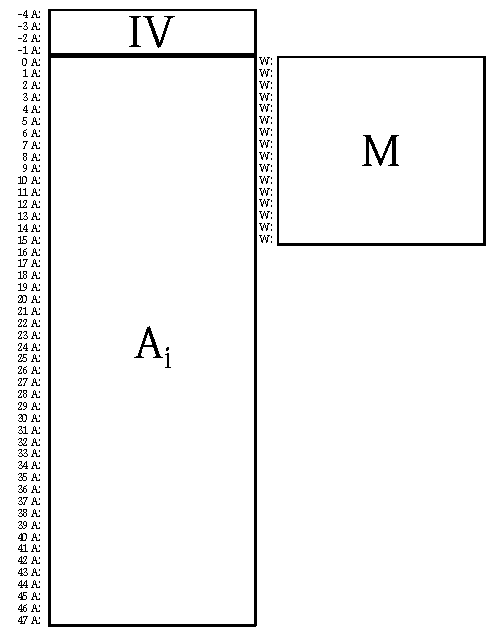
\includegraphics[width=0.4\linewidth]{img/md4_layout.pdf}
    ~~
    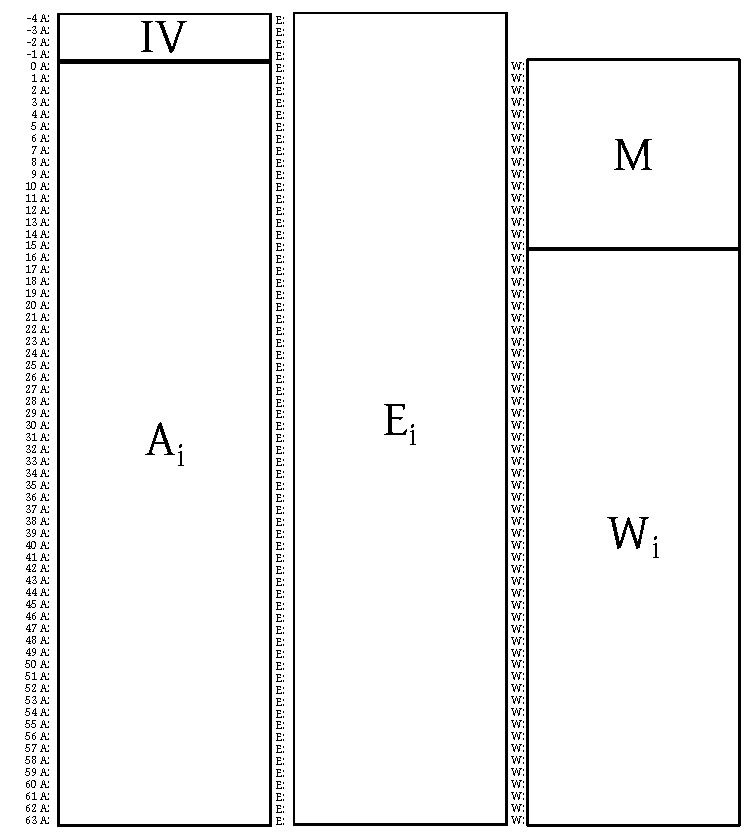
\includegraphics[width=0.5\linewidth]{img/sha256_layout.pdf}
    \caption{Layout of MD4 (left) and SHA-256 (right) differential characteristics}
    \label{img:char-layouts}
  \end{center}
\end{figure}


\texttt{
\begin{table}[p]
\begin{center}
\scalebox{.37}{
\begin{tabular}{|r|c|c|c|c|}
\hline
  $i$  &      &  $\nabla{S_{i,0}}$  &  $\nabla{S_{i,1}}$  &  $\nabla{S_{i,2}}$ \\
\hline
 \dnI{-4} & \dnW: & {{\dnCz}{\dnCo}{\dnCo}{\dnCz}{\dnCz}{\dnCo}{\dnCo}{\dnCo}{\dnCz}{\dnCo}{\dnCz}{\dnCz}{\dnCz}{\dnCo}{\dnCz}{\dnCo}{\dnCz}{\dnCz}{\dnCo}{\dnCz}{\dnCz}{\dnCz}{\dnCo}{\dnCo}{\dnCz}{\dnCz}{\dnCz}{\dnCz}{\dnCz}{\dnCz}{\dnCz}{\dnCo}} & & \\
 \dnI{-3} & \dnW: & {{\dnCz}{\dnCz}{\dnCz}{\dnCo}{\dnCz}{\dnCz}{\dnCz}{\dnCz}{\dnCz}{\dnCz}{\dnCo}{\dnCo}{\dnCz}{\dnCz}{\dnCo}{\dnCz}{\dnCz}{\dnCo}{\dnCz}{\dnCo}{\dnCz}{\dnCo}{\dnCz}{\dnCz}{\dnCz}{\dnCo}{\dnCo}{\dnCo}{\dnCz}{\dnCo}{\dnCo}{\dnCz}} & & \\
 \dnI{-2} & \dnW: & {{\dnCo}{\dnCz}{\dnCz}{\dnCo}{\dnCo}{\dnCz}{\dnCz}{\dnCz}{\dnCo}{\dnCz}{\dnCo}{\dnCo}{\dnCo}{\dnCz}{\dnCo}{\dnCz}{\dnCo}{\dnCo}{\dnCz}{\dnCo}{\dnCo}{\dnCo}{\dnCz}{\dnCz}{\dnCo}{\dnCo}{\dnCo}{\dnCo}{\dnCo}{\dnCo}{\dnCo}{\dnCz}} & & \\
 \dnI{-1} & \dnW: & {{\dnCo}{\dnCo}{\dnCo}{\dnCz}{\dnCo}{\dnCo}{\dnCo}{\dnCo}{\dnCo}{\dnCo}{\dnCz}{\dnCz}{\dnCo}{\dnCo}{\dnCz}{\dnCo}{\dnCo}{\dnCz}{\dnCo}{\dnCz}{\dnCo}{\dnCz}{\dnCo}{\dnCo}{\dnCo}{\dnCz}{\dnCz}{\dnCz}{\dnCo}{\dnCz}{\dnCz}{\dnCo}} & & \\
 \dnI{0} & \dnW: & {{\dnCz}{\dnCo}{\dnCo}{\dnCz}{\dnCo}{\dnCz}{\dnCo}{\dnCo}{\dnCo}{\dnCo}{\dnCz}{\dnCo}{\dnCz}{\dnCo}{\dnCz}{\dnCz}{\dnCo}{\dnCo}{\dnCo}{\dnCz}{\dnCz}{\dnCo}{\dnCz}{\dnCz}{\dnCz}{\dnCz}{\dnCz}{\dnCo}{\dnCz}{\dnCz}{\dnCo}{\dnCz}} & \dnW[W]{}: & {{\dnCz}{\dnCo}{\dnCz}{\dnCz}{\dnCo}{\dnCo}{\dnCz}{\dnCo}{\dnCz}{\dnCo}{\dnCo}{\dnCo}{\dnCo}{\dnCz}{\dnCo}{\dnCz}{\dnCo}{\dnCz}{\dnCz}{\dnCo}{\dnCo}{\dnCo}{\dnCz}{\dnCz}{\dnCo}{\dnCz}{\dnCz}{\dnCz}{\dnCz}{\dnCz}{\dnCo}{\dnCo}} \\
 \dnI{1} & \dnW: & {{\dnCz}{\dnCo}{\dnCo}{\dnCo}{\dnCz}{\dnCo}{\dnCo}{\dnCz}{\dnCz}{\dnCo}{\dnCz}{\dnCz}{\dnCo}{\dnCo}{\dnCo}{\dnCo}{\dnCo}{\dnCo}{\dnCo}{\dnCz}{\dnCo}{\dnCo}{\dnCo}{\dnCz}{\dnCz}{\dnCu}{\dnCo}{\dnCo}{\dnCz}{\dnCz}{\dnCz}{\dnCo}} & \dnW[W]{}: & {{\dnCu}{\dnCo}{\dnCz}{\dnCo}{\dnCz}{\dnCo}{\dnCo}{\dnCz}{\dnCo}{\dnCo}{\dnCz}{\dnCz}{\dnCo}{\dnCz}{\dnCo}{\dnCo}{\dnCo}{\dnCz}{\dnCz}{\dnCo}{\dnCz}{\dnCz}{\dnCo}{\dnCz}{\dnCz}{\dnCo}{\dnCo}{\dnCo}{\dnCo}{\dnCz}{\dnCo}{\dnCz}} \\
 \dnI{2} & \dnW: & {{\dnCo}{\dnCz}{\dnCo}{\dnCz}{\dnCo}{\dnCz}{\dnCo}{\dnCo}{\dnCz}{\dnCo}{\dnCz}{\dnCz}{\dnCz}{\dnCz}{\dnCz}{\dnCz}{\dnCz}{\dnCo}{\dnCo}{\dnCo}{\dnCz}{\dnCu}{\dnCz}{\dnCo}{\dnCn}{\dnCo}{\dnCo}{\dnCo}{\dnCz}{\dnCz}{\dnCo}{\dnCz}} & \dnW[W]{}: & {{\dnCn}{\dnCz}{\dnCo}{\dnCn}{\dnCo}{\dnCz}{\dnCz}{\dnCo}{\dnCo}{\dnCo}{\dnCz}{\dnCo}{\dnCz}{\dnCo}{\dnCz}{\dnCo}{\dnCo}{\dnCz}{\dnCo}{\dnCz}{\dnCz}{\dnCo}{\dnCz}{\dnCo}{\dnCz}{\dnCo}{\dnCo}{\dnCo}{\dnCo}{\dnCz}{\dnCz}{\dnCz}} \\
 \dnI{3} & \dnW: & {{\dnCo}{\dnCz}{\dnCo}{\dnCz}{\dnCo}{\dnCo}{\dnCu}{\dnCo}{\dnCz}{\dnCz}{\dnCo}{\dnCo}{\dnCo}{\dnCo}{\dnCz}{\dnCo}{\dnCz}{\dnCo}{\dnCz}{\dnCo}{\dnCz}{\dnCz}{\dnCo}{\dnCz}{\dnCz}{\dnCo}{\dnCz}{\dnCo}{\dnCz}{\dnCz}{\dnCz}{\dnCo}} & \dnW[W]{}: & {{\dnCz}{\dnCo}{\dnCz}{\dnCo}{\dnCz}{\dnCo}{\dnCo}{\dnCo}{\dnCo}{\dnCz}{\dnCo}{\dnCz}{\dnCz}{\dnCo}{\dnCo}{\dnCo}{\dnCo}{\dnCz}{\dnCo}{\dnCz}{\dnCz}{\dnCo}{\dnCz}{\dnCo}{\dnCo}{\dnCo}{\dnCo}{\dnCz}{\dnCo}{\dnCo}{\dnCo}{\dnCz}} \\
 \dnI{4} & \dnW: & {{\dnCz}{\dnCz}{\dnCo}{\dnCz}{\dnCo}{\dnCo}{\dnCz}{\dnCz}{\dnCz}{\dnCo}{\dnCo}{\dnCz}{\dnCz}{\dnCz}{\dnCo}{\dnCo}{\dnCz}{\dnCo}{\dnCz}{\dnCo}{\dnCz}{\dnCo}{\dnCz}{\dnCo}{\dnCo}{\dnCo}{\dnCo}{\dnCo}{\dnCz}{\dnCz}{\dnCo}{\dnCz}} & \dnW[W]{}: & {{\dnCo}{\dnCo}{\dnCz}{\dnCo}{\dnCo}{\dnCo}{\dnCo}{\dnCz}{\dnCz}{\dnCo}{\dnCo}{\dnCo}{\dnCz}{\dnCo}{\dnCz}{\dnCz}{\dnCo}{\dnCz}{\dnCz}{\dnCz}{\dnCo}{\dnCz}{\dnCo}{\dnCz}{\dnCz}{\dnCz}{\dnCo}{\dnCo}{\dnCo}{\dnCo}{\dnCz}{\dnCz}} \\
 \dnI{5} & \dnW: & {{\dnCz}{\dnCz}{\dnCz}{\dnCo}{\dnCo}{\dnCz}{\dnCo}{\dnCz}{\dnCz}{\dnCo}{\dnCo}{\dnCz}{\dnCz}{\dnCz}{\dnCo}{\dnCz}{\dnCo}{\dnCz}{\dnCu}{\dnCo}{\dnCo}{\dnCz}{\dnCo}{\dnCz}{\dnCz}{\dnCz}{\dnCz}{\dnCz}{\dnCz}{\dnCz}{\dnCz}{\dnCo}} & \dnW[W]{}: & {{\dnCo}{\dnCo}{\dnCz}{\dnCo}{\dnCo}{\dnCo}{\dnCz}{\dnCz}{\dnCo}{\dnCo}{\dnCz}{\dnCz}{\dnCz}{\dnCz}{\dnCo}{\dnCo}{\dnCz}{\dnCo}{\dnCo}{\dnCz}{\dnCz}{\dnCo}{\dnCo}{\dnCz}{\dnCo}{\dnCz}{\dnCo}{\dnCo}{\dnCz}{\dnCz}{\dnCo}{\dnCo}} \\
 \dnI{6} & \dnW: & {{\dnCz}{\dnCz}{\dnCz}{\dnCo}{\dnCo}{\dnCz}{\dnCo}{\dnCo}{\dnCz}{\dnCz}{\dnCu}{\dnCn}{\dnCu}{\dnCu}{\dnCo}{\dnCo}{\dnCz}{\dnCz}{\dnCz}{\dnCo}{\dnCz}{\dnCz}{\dnCz}{\dnCz}{\dnCz}{\dnCo}{\dnCo}{\dnCo}{\dnCo}{\dnCz}{\dnCo}{\dnCz}} & \dnW[W]{}: & {{\dnCq}{\dnCq}{\dnCq}{\dnCq}{\dnCq}{\dnCq}{\dnCq}{\dnCq}{\dnCq}{\dnCq}{\dnCq}{\dnCq}{\dnCq}{\dnCq}{\dnCq}{\dnCq}{\dnCq}{\dnCq}{\dnCq}{\dnCq}{\dnCq}{\dnCq}{\dnCq}{\dnCq}{\dnCq}{\dnCq}{\dnCq}{\dnCq}{\dnCq}{\dnCq}{\dnCq}{\dnCq}} \\
 \dnI{7} & \dnW: & {{\dnCz}{\dnCz}{\dnCo}{\dnCz}{\dnCo}{\dnCz}{\dnCo}{\dnCo}{\dnCo}{\dnCz}{\dnCz}{\dnCz}{\dnCz}{\dnCz}{\dnCz}{\dnCo}{\dnCz}{\dnCu}{\dnCn}{\dnCn}{\dnCz}{\dnCo}{\dnCo}{\dnCz}{\dnCz}{\dnCo}{\dnCz}{\dnCo}{\dnCz}{\dnCz}{\dnCz}{\dnCz}} & \dnW[W]{}: & {{\dnCz}{\dnCz}{\dnCo}{\dnCo}{\dnCo}{\dnCz}{\dnCo}{\dnCo}{\dnCz}{\dnCz}{\dnCo}{\dnCz}{\dnCo}{\dnCz}{\dnCo}{\dnCz}{\dnCz}{\dnCo}{\dnCz}{\dnCo}{\dnCo}{\dnCo}{\dnCz}{\dnCo}{\dnCo}{\dnCz}{\dnCz}{\dnCo}{\dnCo}{\dnCo}{\dnCo}{\dnCo}} \\
 \dnI{8} & \dnW: & {{\dnCq}{\dnCq}{\dnCq}{\dnCq}{\dnCq}{\dnCq}{\dnCq}{\dnCq}{\dnCq}{\dnCq}{\dnCq}{\dnCq}{\dnCq}{\dnCq}{\dnCq}{\dnCq}{\dnCq}{\dnCq}{\dnCq}{\dnCq}{\dnCq}{\dnCq}{\dnCq}{\dnCq}{\dnCq}{\dnCq}{\dnCq}{\dnCq}{\dnCq}{\dnCq}{\dnCq}{\dnCq}} & \dnW[W]{}: & {{\dnCo}{\dnCo}{\dnCz}{\dnCz}{\dnCz}{\dnCo}{\dnCo}{\dnCz}{\dnCo}{\dnCz}{\dnCz}{\dnCo}{\dnCo}{\dnCo}{\dnCz}{\dnCo}{\dnCz}{\dnCo}{\dnCo}{\dnCo}{\dnCz}{\dnCz}{\dnCz}{\dnCo}{\dnCo}{\dnCz}{\dnCo}{\dnCo}{\dnCz}{\dnCz}{\dnCo}{\dnCo}} \\
 \dnI{9} & \dnW: & {{\dnCq}{\dnCq}{\dnCq}{\dnCq}{\dnCq}{\dnCq}{\dnCq}{\dnCq}{\dnCq}{\dnCq}{\dnCq}{\dnCq}{\dnCq}{\dnCq}{\dnCq}{\dnCq}{\dnCq}{\dnCq}{\dnCq}{\dnCq}{\dnCq}{\dnCq}{\dnCq}{\dnCq}{\dnCq}{\dnCq}{\dnCq}{\dnCq}{\dnCq}{\dnCq}{\dnCq}{\dnCq}} & \dnW[W]{}: & {{\dnCo}{\dnCo}{\dnCo}{\dnCo}{\dnCo}{\dnCz}{\dnCz}{\dnCo}{\dnCo}{\dnCo}{\dnCo}{\dnCz}{\dnCo}{\dnCz}{\dnCz}{\dnCo}{\dnCo}{\dnCz}{\dnCz}{\dnCo}{\dnCz}{\dnCz}{\dnCz}{\dnCo}{\dnCo}{\dnCz}{\dnCz}{\dnCo}{\dnCo}{\dnCz}{\dnCz}{\dnCz}} \\
 \dnI{10} & \dnW: & {{\dnCo}{\dnCz}{\dnCn}{\dnCz}{\dnCz}{\dnCo}{\dnCz}{\dnCz}{\dnCo}{\dnCz}{\dnCz}{\dnCz}{\dnCz}{\dnCo}{\dnCz}{\dnCo}{\dnCq}{\dnCq}{\dnCq}{\dnCq}{\dnCq}{\dnCq}{\dnCq}{\dnCq}{\dnCq}{\dnCq}{\dnCq}{\dnCq}{\dnCq}{\dnCo}{\dnCo}{\dnCz}} & \dnW[W]{}: & {{\dnCo}{\dnCo}{\dnCz}{\dnCo}{\dnCz}{\dnCo}{\dnCo}{\dnCo}{\dnCo}{\dnCz}{\dnCz}{\dnCo}{\dnCo}{\dnCo}{\dnCo}{\dnCo}{\dnCo}{\dnCz}{\dnCz}{\dnCz}{\dnCz}{\dnCz}{\dnCz}{\dnCz}{\dnCz}{\dnCo}{\dnCz}{\dnCo}{\dnCo}{\dnCo}{\dnCo}{\dnCz}} \\
 \dnI{11} & \dnW: & {{\dnCu}{\dnCo}{\dnCz}{\dnCz}{\dnCz}{\dnCo}{\dnCo}{\dnCz}{\dnCo}{\dnCz}{\dnCo}{\dnCo}{\dnCz}{\dnCo}{\dnCo}{\dnCz}{\dnCq}{\dnCq}{\dnCq}{\dnCq}{\dnCq}{\dnCq}{\dnCq}{\dnCq}{\dnCq}{\dnCq}{\dnCq}{\dnCq}{\dnCq}{\dnCo}{\dnCo}{\dnCo}} & \dnW[W]{}: & {{\dnCo}{\dnCz}{\dnCo}{\dnCz}{\dnCz}{\dnCo}{\dnCo}{\dnCz}{\dnCz}{\dnCz}{\dnCo}{\dnCo}{\dnCo}{\dnCz}{\dnCo}{\dnCo}{\dnCo}{\dnCz}{\dnCo}{\dnCo}{\dnCz}{\dnCz}{\dnCo}{\dnCz}{\dnCo}{\dnCo}{\dnCo}{\dnCz}{\dnCo}{\dnCz}{\dnCz}{\dnCz}} \\
 \dnI{12} & \dnW: & {{\dnCz}{\dnCz}{\dnCo}{\dnCz}{\dnCo}{\dnCo}{\dnCu}{\dnCz}{\dnCz}{\dnCu}{\dnCo}{\dnCz}{\dnCo}{\dnCz}{\dnCo}{\dnCo}{\dnCq}{\dnCq}{\dnCq}{\dnCq}{\dnCq}{\dnCq}{\dnCq}{\dnCq}{\dnCq}{\dnCq}{\dnCq}{\dnCq}{\dnCq}{\dnCz}{\dnCo}{\dnCo}} & \dnW[W]{}: & {{\dnCz}{\dnCo}{\dnCz}{\dnCz}{\dnCz}{\dnCo}{\dnCz}{\dnCo}{\dnCo}{\dnCo}{\dnCz}{\dnCo}{\dnCo}{\dnCo}{\dnCz}{\dnCn}{\dnCo}{\dnCz}{\dnCz}{\dnCz}{\dnCo}{\dnCo}{\dnCo}{\dnCz}{\dnCz}{\dnCz}{\dnCo}{\dnCo}{\dnCz}{\dnCz}{\dnCz}{\dnCo}} \\
 \dnI{13} & \dnW: & {{\dnCo}{\dnCz}{\dnCu}{\dnCn}{\dnCo}{\dnCn}{\dnCz}{\dnCo}{\dnCz}{\dnCz}{\dnCo}{\dnCo}{\dnCz}{\dnCz}{\dnCz}{\dnCo}{\dnCq}{\dnCq}{\dnCq}{\dnCq}{\dnCq}{\dnCq}{\dnCq}{\dnCq}{\dnCq}{\dnCq}{\dnCq}{\dnCq}{\dnCq}{\dnCo}{\dnCz}{\dnCo}} & \dnW[W]{}: & {{\dnCo}{\dnCz}{\dnCz}{\dnCo}{\dnCz}{\dnCo}{\dnCo}{\dnCo}{\dnCo}{\dnCo}{\dnCo}{\dnCz}{\dnCz}{\dnCz}{\dnCo}{\dnCo}{\dnCz}{\dnCz}{\dnCz}{\dnCo}{\dnCo}{\dnCo}{\dnCo}{\dnCo}{\dnCo}{\dnCo}{\dnCo}{\dnCz}{\dnCz}{\dnCo}{\dnCz}{\dnCo}} \\
 \dnI{14} & \dnW: & {{\dnCz}{\dnCz}{\dnCz}{\dnCz}{\dnCo}{\dnCz}{\dnCo}{\dnCz}{\dnCz}{\dnCo}{\dnCz}{\dnCo}{\dnCz}{\dnCz}{\dnCz}{\dnCo}{\dnCh}{\dnCh}{\dnCh}{\dnCh}{\dnCh}{\dnCh}{\dnCh}{\dnCh}{\dnCh}{\dnCh}{\dnCh}{\dnCh}{\dnCh}{\dnCo}{\dnCo}{\dnCz}} & \dnW[W]{}: & {{\dnCz}{\dnCz}{\dnCo}{\dnCz}{\dnCz}{\dnCo}{\dnCo}{\dnCo}{\dnCo}{\dnCz}{\dnCz}{\dnCo}{\dnCz}{\dnCo}{\dnCz}{\dnCz}{\dnCo}{\dnCz}{\dnCo}{\dnCo}{\dnCo}{\dnCo}{\dnCo}{\dnCo}{\dnCz}{\dnCz}{\dnCz}{\dnCz}{\dnCo}{\dnCz}{\dnCz}{\dnCz}} \\
 \dnI{15} & \dnW: & {{\dnCz}{\dnCz}{\dnCz}{\dnCo}{\dnCo}{\dnCo}{\dnCo}{\dnCz}{\dnCo}{\dnCz}{\dnCo}{\dnCz}{\dnCo}{\dnCu}{\dnCz}{\dnCo}{\dnCh}{\dnCh}{\dnCh}{\dnCh}{\dnCh}{\dnCh}{\dnCh}{\dnCh}{\dnCh}{\dnCh}{\dnCh}{\dnCh}{\dnCh}{\dnCo}{\dnCz}{\dnCz}} & \dnW[W]{}: & {{\dnCo}{\dnCz}{\dnCo}{\dnCo}{\dnCo}{\dnCz}{\dnCz}{\dnCo}{\dnCo}{\dnCo}{\dnCo}{\dnCz}{\dnCo}{\dnCz}{\dnCz}{\dnCz}{\dnCo}{\dnCo}{\dnCz}{\dnCz}{\dnCz}{\dnCz}{\dnCo}{\dnCo}{\dnCo}{\dnCo}{\dnCo}{\dnCz}{\dnCo}{\dnCz}{\dnCz}{\dnCo}} \\
 \dnI{16} & \dnW: & {{\dnCn}{\dnCz}{\dnCz}{\dnCn}{\dnCz}{\dnCu}{\dnCn}{\dnCz}{\dnCo}{\dnCo}{\dnCz}{\dnCo}{\dnCz}{\dnCz}{\dnCo}{\dnCz}{\dnCh}{\dnCh}{\dnCh}{\dnCh}{\dnCh}{\dnCh}{\dnCh}{\dnCh}{\dnCh}{\dnCh}{\dnCh}{\dnCh}{\dnCh}{\dnCo}{\dnCo}{\dnCo}} & & \\
 \dnI{17} & \dnW: & {{\dnCz}{\dnCz}{\dnCz}{\dnCo}{\dnCo}{\dnCo}{\dnCo}{\dnCo}{\dnCz}{\dnCz}{\dnCo}{\dnCo}{\dnCo}{\dnCz}{\dnCo}{\dnCz}{\dnCh}{\dnCh}{\dnCh}{\dnCh}{\dnCh}{\dnCh}{\dnCh}{\dnCh}{\dnCh}{\dnCh}{\dnCh}{\dnCh}{\dnCh}{\dnCo}{\dnCo}{\dnCz}} & & \\
 \dnI{18} & \dnW: & {{\dnCz}{\dnCo}{\dnCz}{\dnCo}{\dnCz}{\dnCo}{\dnCo}{\dnCo}{\dnCz}{\dnCz}{\dnCz}{\dnCz}{\dnCo}{\dnCo}{\dnCz}{\dnCo}{\dnCh}{\dnCh}{\dnCh}{\dnCh}{\dnCh}{\dnCh}{\dnCh}{\dnCh}{\dnCh}{\dnCh}{\dnCh}{\dnCh}{\dnCh}{\dnCo}{\dnCz}{\dnCz}} & & \\
 \dnI{19} & \dnW: & {{\dnCu}{\dnCo}{\dnCn}{\dnCo}{\dnCz}{\dnCz}{\dnCz}{\dnCz}{\dnCz}{\dnCz}{\dnCz}{\dnCo}{\dnCz}{\dnCo}{\dnCo}{\dnCo}{\dnCh}{\dnCh}{\dnCh}{\dnCh}{\dnCh}{\dnCh}{\dnCh}{\dnCh}{\dnCh}{\dnCh}{\dnCh}{\dnCh}{\dnCh}{\dnCo}{\dnCz}{\dnCz}} & & \\
 \dnI{20} & \dnW: & {{\dnCn}{\dnCo}{\dnCu}{\dnCn}{\dnCo}{\dnCz}{\dnCz}{\dnCo}{\dnCo}{\dnCo}{\dnCo}{\dnCo}{\dnCo}{\dnCo}{\dnCz}{\dnCo}{\dnCo}{\dnCo}{\dnCz}{\dnCo}{\dnCz}{\dnCz}{\dnCz}{\dnCz}{\dnCz}{\dnCz}{\dnCo}{\dnCo}{\dnCz}{\dnCo}{\dnCz}{\dnCz}} & & \\
 \dnI{21} & \dnW: & {{\dnCo}{\dnCo}{\dnCo}{\dnCo}{\dnCz}{\dnCz}{\dnCo}{\dnCo}{\dnCo}{\dnCz}{\dnCo}{\dnCo}{\dnCz}{\dnCz}{\dnCz}{\dnCz}{\dnCz}{\dnCo}{\dnCz}{\dnCo}{\dnCo}{\dnCo}{\dnCo}{\dnCo}{\dnCo}{\dnCo}{\dnCz}{\dnCo}{\dnCz}{\dnCo}{\dnCz}{\dnCz}} & & \\
 \dnI{22} & \dnW: & {{\dnCz}{\dnCo}{\dnCz}{\dnCo}{\dnCo}{\dnCo}{\dnCz}{\dnCo}{\dnCo}{\dnCo}{\dnCz}{\dnCz}{\dnCo}{\dnCo}{\dnCz}{\dnCo}{\dnCz}{\dnCz}{\dnCo}{\dnCo}{\dnCz}{\dnCz}{\dnCo}{\dnCo}{\dnCz}{\dnCz}{\dnCo}{\dnCo}{\dnCo}{\dnCz}{\dnCo}{\dnCz}} & & \\
 \dnI{23} & \dnW: & {{\dnCz}{\dnCo}{\dnCz}{\dnCo}{\dnCz}{\dnCz}{\dnCz}{\dnCz}{\dnCo}{\dnCo}{\dnCo}{\dnCz}{\dnCo}{\dnCo}{\dnCo}{\dnCz}{\dnCo}{\dnCo}{\dnCz}{\dnCz}{\dnCz}{\dnCo}{\dnCo}{\dnCo}{\dnCo}{\dnCz}{\dnCz}{\dnCz}{\dnCo}{\dnCo}{\dnCo}{\dnCo}} & & \\
 \dnI{24} & \dnW: & {{\dnCz}{\dnCz}{\dnCz}{\dnCz}{\dnCz}{\dnCz}{\dnCo}{\dnCz}{\dnCz}{\dnCz}{\dnCz}{\dnCo}{\dnCz}{\dnCz}{\dnCo}{\dnCz}{\dnCz}{\dnCz}{\dnCo}{\dnCo}{\dnCz}{\dnCo}{\dnCo}{\dnCo}{\dnCz}{\dnCz}{\dnCz}{\dnCo}{\dnCo}{\dnCz}{\dnCo}{\dnCz}} & & \\
 \dnI{25} & \dnW: & {{\dnCo}{\dnCz}{\dnCo}{\dnCo}{\dnCz}{\dnCz}{\dnCz}{\dnCz}{\dnCo}{\dnCz}{\dnCz}{\dnCo}{\dnCz}{\dnCo}{\dnCo}{\dnCz}{\dnCz}{\dnCz}{\dnCz}{\dnCo}{\dnCz}{\dnCo}{\dnCz}{\dnCz}{\dnCo}{\dnCo}{\dnCo}{\dnCz}{\dnCo}{\dnCz}{\dnCo}{\dnCz}} & & \\
 \dnI{26} & \dnW: & {{\dnCz}{\dnCz}{\dnCz}{\dnCz}{\dnCo}{\dnCz}{\dnCo}{\dnCz}{\dnCo}{\dnCz}{\dnCz}{\dnCz}{\dnCo}{\dnCz}{\dnCz}{\dnCo}{\dnCz}{\dnCo}{\dnCo}{\dnCo}{\dnCz}{\dnCo}{\dnCo}{\dnCo}{\dnCz}{\dnCo}{\dnCz}{\dnCz}{\dnCz}{\dnCz}{\dnCz}{\dnCo}} & & \\
 \dnI{27} & \dnW: & {{\dnCz}{\dnCz}{\dnCz}{\dnCz}{\dnCz}{\dnCo}{\dnCo}{\dnCz}{\dnCo}{\dnCo}{\dnCo}{\dnCz}{\dnCo}{\dnCo}{\dnCo}{\dnCo}{\dnCz}{\dnCo}{\dnCz}{\dnCo}{\dnCo}{\dnCz}{\dnCo}{\dnCz}{\dnCo}{\dnCz}{\dnCo}{\dnCo}{\dnCz}{\dnCz}{\dnCo}{\dnCo}} & & \\
 \dnI{28} & \dnW: & {{\dnCo}{\dnCz}{\dnCo}{\dnCo}{\dnCz}{\dnCo}{\dnCo}{\dnCz}{\dnCz}{\dnCo}{\dnCz}{\dnCo}{\dnCo}{\dnCo}{\dnCz}{\dnCo}{\dnCz}{\dnCo}{\dnCo}{\dnCz}{\dnCo}{\dnCo}{\dnCz}{\dnCz}{\dnCz}{\dnCz}{\dnCo}{\dnCz}{\dnCz}{\dnCo}{\dnCz}{\dnCo}} & & \\
 \dnI{29} & \dnW: & {{\dnCo}{\dnCz}{\dnCo}{\dnCz}{\dnCz}{\dnCz}{\dnCo}{\dnCz}{\dnCz}{\dnCz}{\dnCz}{\dnCz}{\dnCo}{\dnCo}{\dnCz}{\dnCo}{\dnCz}{\dnCo}{\dnCz}{\dnCz}{\dnCo}{\dnCz}{\dnCz}{\dnCz}{\dnCz}{\dnCo}{\dnCo}{\dnCz}{\dnCo}{\dnCz}{\dnCz}{\dnCo}} & & \\
 \dnI{30} & \dnW: & {{\dnCz}{\dnCz}{\dnCo}{\dnCz}{\dnCo}{\dnCz}{\dnCz}{\dnCo}{\dnCo}{\dnCo}{\dnCz}{\dnCo}{\dnCz}{\dnCo}{\dnCo}{\dnCo}{\dnCo}{\dnCo}{\dnCz}{\dnCz}{\dnCz}{\dnCo}{\dnCo}{\dnCo}{\dnCz}{\dnCo}{\dnCo}{\dnCz}{\dnCz}{\dnCz}{\dnCo}{\dnCo}} & & \\
 \dnI{31} & \dnW: & {{\dnCo}{\dnCo}{\dnCo}{\dnCo}{\dnCo}{\dnCo}{\dnCz}{\dnCz}{\dnCo}{\dnCz}{\dnCz}{\dnCo}{\dnCz}{\dnCz}{\dnCo}{\dnCz}{\dnCo}{\dnCo}{\dnCz}{\dnCo}{\dnCz}{\dnCo}{\dnCo}{\dnCo}{\dnCo}{\dnCz}{\dnCo}{\dnCo}{\dnCz}{\dnCo}{\dnCo}{\dnCz}} & & \\
 \dnI{32} & \dnW: & {{\dnCz}{\dnCo}{\dnCz}{\dnCz}{\dnCo}{\dnCo}{\dnCo}{\dnCo}{\dnCo}{\dnCo}{\dnCz}{\dnCo}{\dnCz}{\dnCz}{\dnCo}{\dnCz}{\dnCz}{\dnCo}{\dnCo}{\dnCz}{\dnCo}{\dnCz}{\dnCz}{\dnCz}{\dnCz}{\dnCz}{\dnCo}{\dnCz}{\dnCo}{\dnCo}{\dnCo}{\dnCo}} & & \\
 \dnI{33} & \dnW: & {{\dnCz}{\dnCz}{\dnCo}{\dnCo}{\dnCo}{\dnCz}{\dnCz}{\dnCz}{\dnCz}{\dnCz}{\dnCo}{\dnCo}{\dnCo}{\dnCo}{\dnCz}{\dnCo}{\dnCz}{\dnCo}{\dnCo}{\dnCz}{\dnCo}{\dnCo}{\dnCo}{\dnCz}{\dnCo}{\dnCo}{\dnCo}{\dnCz}{\dnCz}{\dnCo}{\dnCz}{\dnCz}} & & \\
 \dnI{34} & \dnW: & {{\dnCz}{\dnCz}{\dnCo}{\dnCz}{\dnCz}{\dnCz}{\dnCz}{\dnCz}{\dnCz}{\dnCo}{\dnCo}{\dnCo}{\dnCz}{\dnCo}{\dnCz}{\dnCo}{\dnCo}{\dnCo}{\dnCo}{\dnCz}{\dnCo}{\dnCz}{\dnCz}{\dnCz}{\dnCz}{\dnCz}{\dnCz}{\dnCo}{\dnCz}{\dnCo}{\dnCz}{\dnCo}} & & \\
 \dnI{35} & \dnW: & {{\dnCn}{\dnCz}{\dnCo}{\dnCz}{\dnCz}{\dnCz}{\dnCz}{\dnCz}{\dnCz}{\dnCz}{\dnCo}{\dnCo}{\dnCz}{\dnCz}{\dnCo}{\dnCo}{\dnCz}{\dnCz}{\dnCz}{\dnCz}{\dnCz}{\dnCo}{\dnCz}{\dnCz}{\dnCz}{\dnCo}{\dnCo}{\dnCo}{\dnCz}{\dnCz}{\dnCo}{\dnCz}} & & \\
 \dnI{36} & \dnW: & {{\dnCn}{\dnCz}{\dnCz}{\dnCz}{\dnCz}{\dnCo}{\dnCo}{\dnCo}{\dnCo}{\dnCo}{\dnCo}{\dnCz}{\dnCo}{\dnCz}{\dnCo}{\dnCo}{\dnCo}{\dnCo}{\dnCz}{\dnCo}{\dnCo}{\dnCo}{\dnCo}{\dnCz}{\dnCz}{\dnCo}{\dnCz}{\dnCo}{\dnCo}{\dnCz}{\dnCz}{\dnCo}} & & \\
 \dnI{37} & \dnW: & {{\dnCo}{\dnCo}{\dnCz}{\dnCz}{\dnCo}{\dnCz}{\dnCz}{\dnCz}{\dnCz}{\dnCz}{\dnCz}{\dnCo}{\dnCo}{\dnCz}{\dnCo}{\dnCz}{\dnCz}{\dnCo}{\dnCz}{\dnCz}{\dnCz}{\dnCz}{\dnCo}{\dnCo}{\dnCz}{\dnCz}{\dnCz}{\dnCz}{\dnCo}{\dnCo}{\dnCz}{\dnCz}} & & \\
 \dnI{38} & \dnW: & {{\dnCo}{\dnCz}{\dnCo}{\dnCo}{\dnCz}{\dnCz}{\dnCz}{\dnCz}{\dnCz}{\dnCo}{\dnCo}{\dnCz}{\dnCz}{\dnCo}{\dnCo}{\dnCo}{\dnCo}{\dnCo}{\dnCo}{\dnCz}{\dnCo}{\dnCz}{\dnCz}{\dnCo}{\dnCo}{\dnCz}{\dnCo}{\dnCz}{\dnCo}{\dnCo}{\dnCz}{\dnCz}} & & \\
 \dnI{39} & \dnW: & {{\dnCz}{\dnCz}{\dnCz}{\dnCo}{\dnCz}{\dnCz}{\dnCo}{\dnCz}{\dnCz}{\dnCz}{\dnCz}{\dnCz}{\dnCo}{\dnCz}{\dnCo}{\dnCz}{\dnCz}{\dnCz}{\dnCz}{\dnCo}{\dnCo}{\dnCz}{\dnCo}{\dnCo}{\dnCz}{\dnCz}{\dnCz}{\dnCo}{\dnCo}{\dnCo}{\dnCz}{\dnCz}} & & \\
 \dnI{40} & \dnW: & {{\dnCo}{\dnCo}{\dnCz}{\dnCz}{\dnCz}{\dnCz}{\dnCz}{\dnCz}{\dnCz}{\dnCo}{\dnCz}{\dnCz}{\dnCo}{\dnCz}{\dnCz}{\dnCz}{\dnCz}{\dnCo}{\dnCo}{\dnCo}{\dnCz}{\dnCz}{\dnCz}{\dnCo}{\dnCo}{\dnCz}{\dnCz}{\dnCz}{\dnCz}{\dnCo}{\dnCz}{\dnCo}} & & \\
 \dnI{41} & \dnW: & {{\dnCz}{\dnCz}{\dnCz}{\dnCz}{\dnCz}{\dnCo}{\dnCo}{\dnCz}{\dnCo}{\dnCz}{\dnCz}{\dnCz}{\dnCz}{\dnCo}{\dnCo}{\dnCz}{\dnCo}{\dnCo}{\dnCo}{\dnCo}{\dnCz}{\dnCo}{\dnCz}{\dnCo}{\dnCz}{\dnCz}{\dnCo}{\dnCz}{\dnCz}{\dnCo}{\dnCo}{\dnCz}} & & \\
 \dnI{42} & \dnW: & {{\dnCz}{\dnCo}{\dnCz}{\dnCz}{\dnCo}{\dnCo}{\dnCo}{\dnCz}{\dnCo}{\dnCo}{\dnCz}{\dnCo}{\dnCo}{\dnCo}{\dnCz}{\dnCo}{\dnCo}{\dnCo}{\dnCo}{\dnCo}{\dnCo}{\dnCo}{\dnCo}{\dnCz}{\dnCo}{\dnCz}{\dnCz}{\dnCz}{\dnCz}{\dnCo}{\dnCo}{\dnCz}} & & \\
 \dnI{43} & \dnW: & {{\dnCz}{\dnCo}{\dnCz}{\dnCo}{\dnCz}{\dnCz}{\dnCz}{\dnCz}{\dnCz}{\dnCo}{\dnCo}{\dnCz}{\dnCz}{\dnCz}{\dnCo}{\dnCo}{\dnCo}{\dnCo}{\dnCz}{\dnCo}{\dnCz}{\dnCz}{\dnCz}{\dnCz}{\dnCz}{\dnCo}{\dnCo}{\dnCz}{\dnCo}{\dnCo}{\dnCz}{\dnCo}} & & \\
 \dnI{44} & \dnW: & {{\dnCo}{\dnCo}{\dnCo}{\dnCo}{\dnCo}{\dnCz}{\dnCz}{\dnCz}{\dnCz}{\dnCz}{\dnCz}{\dnCo}{\dnCz}{\dnCo}{\dnCo}{\dnCz}{\dnCo}{\dnCo}{\dnCo}{\dnCo}{\dnCz}{\dnCo}{\dnCo}{\dnCo}{\dnCz}{\dnCz}{\dnCz}{\dnCz}{\dnCo}{\dnCo}{\dnCz}{\dnCz}} & & \\
 \dnI{45} & \dnW: & {{\dnCo}{\dnCz}{\dnCz}{\dnCz}{\dnCo}{\dnCz}{\dnCo}{\dnCz}{\dnCo}{\dnCo}{\dnCz}{\dnCo}{\dnCo}{\dnCz}{\dnCo}{\dnCo}{\dnCz}{\dnCz}{\dnCo}{\dnCz}{\dnCo}{\dnCo}{\dnCz}{\dnCz}{\dnCz}{\dnCz}{\dnCz}{\dnCz}{\dnCz}{\dnCo}{\dnCz}{\dnCz}} & & \\
 \dnI{46} & \dnW: & {{\dnCo}{\dnCz}{\dnCz}{\dnCz}{\dnCz}{\dnCz}{\dnCo}{\dnCz}{\dnCo}{\dnCz}{\dnCz}{\dnCo}{\dnCo}{\dnCz}{\dnCz}{\dnCo}{\dnCz}{\dnCo}{\dnCz}{\dnCo}{\dnCo}{\dnCz}{\dnCz}{\dnCz}{\dnCo}{\dnCo}{\dnCz}{\dnCo}{\dnCo}{\dnCo}{\dnCz}{\dnCz}} & & \\
 \dnI{47} & \dnW: & {{\dnCo}{\dnCz}{\dnCz}{\dnCz}{\dnCz}{\dnCz}{\dnCz}{\dnCo}{\dnCo}{\dnCo}{\dnCo}{\dnCz}{\dnCz}{\dnCo}{\dnCz}{\dnCo}{\dnCo}{\dnCz}{\dnCo}{\dnCo}{\dnCz}{\dnCo}{\dnCz}{\dnCz}{\dnCo}{\dnCz}{\dnCo}{\dnCo}{\dnCo}{\dnCo}{\dnCz}{\dnCo}} & & \\
\hline
\end{tabular}
\hspace{10pt}$\Rightarrow$\hspace{10pt}
\begin{tabular}{|r|c|c|c|c|}
\hline
  $i$  &      &  $\nabla{S_{i,0}}$  &  $\nabla{S_{i,1}}$  &  $\nabla{S_{i,2}}$ \\
\hline
 \dnI{-4} & \dnW: & {{\dnCz}{\dnCo}{\dnCo}{\dnCz}{\dnCz}{\dnCo}{\dnCo}{\dnCo}{\dnCz}{\dnCo}{\dnCz}{\dnCz}{\dnCz}{\dnCo}{\dnCz}{\dnCo}{\dnCz}{\dnCz}{\dnCo}{\dnCz}{\dnCz}{\dnCz}{\dnCo}{\dnCo}{\dnCz}{\dnCz}{\dnCz}{\dnCz}{\dnCz}{\dnCz}{\dnCz}{\dnCo}} & & \\
 \dnI{-3} & \dnW: & {{\dnCz}{\dnCz}{\dnCz}{\dnCo}{\dnCz}{\dnCz}{\dnCz}{\dnCz}{\dnCz}{\dnCz}{\dnCo}{\dnCo}{\dnCz}{\dnCz}{\dnCo}{\dnCz}{\dnCz}{\dnCo}{\dnCz}{\dnCo}{\dnCz}{\dnCo}{\dnCz}{\dnCz}{\dnCz}{\dnCo}{\dnCo}{\dnCo}{\dnCz}{\dnCo}{\dnCo}{\dnCz}} & & \\
 \dnI{-2} & \dnW: & {{\dnCo}{\dnCz}{\dnCz}{\dnCo}{\dnCo}{\dnCz}{\dnCz}{\dnCz}{\dnCo}{\dnCz}{\dnCo}{\dnCo}{\dnCo}{\dnCz}{\dnCo}{\dnCz}{\dnCo}{\dnCo}{\dnCz}{\dnCo}{\dnCo}{\dnCo}{\dnCz}{\dnCz}{\dnCo}{\dnCo}{\dnCo}{\dnCo}{\dnCo}{\dnCo}{\dnCo}{\dnCz}} & & \\
 \dnI{-1} & \dnW: & {{\dnCo}{\dnCo}{\dnCo}{\dnCz}{\dnCo}{\dnCo}{\dnCo}{\dnCo}{\dnCo}{\dnCo}{\dnCz}{\dnCz}{\dnCo}{\dnCo}{\dnCz}{\dnCo}{\dnCo}{\dnCz}{\dnCo}{\dnCz}{\dnCo}{\dnCz}{\dnCo}{\dnCo}{\dnCo}{\dnCz}{\dnCz}{\dnCz}{\dnCo}{\dnCz}{\dnCz}{\dnCo}} & & \\
 \dnI{0} & \dnW: & {{\dnCz}{\dnCo}{\dnCo}{\dnCz}{\dnCo}{\dnCz}{\dnCo}{\dnCo}{\dnCo}{\dnCo}{\dnCz}{\dnCo}{\dnCz}{\dnCo}{\dnCz}{\dnCz}{\dnCo}{\dnCo}{\dnCo}{\dnCz}{\dnCz}{\dnCo}{\dnCz}{\dnCz}{\dnCz}{\dnCz}{\dnCz}{\dnCo}{\dnCz}{\dnCz}{\dnCo}{\dnCz}} & \dnW[W]{}: & {{\dnCz}{\dnCo}{\dnCz}{\dnCz}{\dnCo}{\dnCo}{\dnCz}{\dnCo}{\dnCz}{\dnCo}{\dnCo}{\dnCo}{\dnCo}{\dnCz}{\dnCo}{\dnCz}{\dnCo}{\dnCz}{\dnCz}{\dnCo}{\dnCo}{\dnCo}{\dnCz}{\dnCz}{\dnCo}{\dnCz}{\dnCz}{\dnCz}{\dnCz}{\dnCz}{\dnCo}{\dnCo}} \\
 \dnI{1} & \dnW: & {{\dnCz}{\dnCo}{\dnCo}{\dnCo}{\dnCz}{\dnCo}{\dnCo}{\dnCz}{\dnCz}{\dnCo}{\dnCz}{\dnCz}{\dnCo}{\dnCo}{\dnCo}{\dnCo}{\dnCo}{\dnCo}{\dnCo}{\dnCz}{\dnCo}{\dnCo}{\dnCo}{\dnCz}{\dnCz}{\dnCu}{\dnCo}{\dnCo}{\dnCz}{\dnCz}{\dnCz}{\dnCo}} & \dnW[W]{}: & {{\dnCu}{\dnCo}{\dnCz}{\dnCo}{\dnCz}{\dnCo}{\dnCo}{\dnCz}{\dnCo}{\dnCo}{\dnCz}{\dnCz}{\dnCo}{\dnCz}{\dnCo}{\dnCo}{\dnCo}{\dnCz}{\dnCz}{\dnCo}{\dnCz}{\dnCz}{\dnCo}{\dnCz}{\dnCz}{\dnCo}{\dnCo}{\dnCo}{\dnCo}{\dnCz}{\dnCo}{\dnCz}} \\
 \dnI{2} & \dnW: & {{\dnCo}{\dnCz}{\dnCo}{\dnCz}{\dnCo}{\dnCz}{\dnCo}{\dnCo}{\dnCz}{\dnCo}{\dnCz}{\dnCz}{\dnCz}{\dnCz}{\dnCz}{\dnCz}{\dnCz}{\dnCo}{\dnCo}{\dnCo}{\dnCz}{\dnCu}{\dnCz}{\dnCo}{\dnCn}{\dnCo}{\dnCo}{\dnCo}{\dnCz}{\dnCz}{\dnCo}{\dnCz}} & \dnW[W]{}: & {{\dnCn}{\dnCz}{\dnCo}{\dnCn}{\dnCo}{\dnCz}{\dnCz}{\dnCo}{\dnCo}{\dnCo}{\dnCz}{\dnCo}{\dnCz}{\dnCo}{\dnCz}{\dnCo}{\dnCo}{\dnCz}{\dnCo}{\dnCz}{\dnCz}{\dnCo}{\dnCz}{\dnCo}{\dnCz}{\dnCo}{\dnCo}{\dnCo}{\dnCo}{\dnCz}{\dnCz}{\dnCz}} \\
 \dnI{3} & \dnW: & {{\dnCo}{\dnCz}{\dnCo}{\dnCz}{\dnCo}{\dnCo}{\dnCu}{\dnCo}{\dnCz}{\dnCz}{\dnCo}{\dnCo}{\dnCo}{\dnCo}{\dnCz}{\dnCo}{\dnCz}{\dnCo}{\dnCz}{\dnCo}{\dnCz}{\dnCz}{\dnCo}{\dnCz}{\dnCz}{\dnCo}{\dnCz}{\dnCo}{\dnCz}{\dnCz}{\dnCz}{\dnCo}} & \dnW[W]{}: & {{\dnCz}{\dnCo}{\dnCz}{\dnCo}{\dnCz}{\dnCo}{\dnCo}{\dnCo}{\dnCo}{\dnCz}{\dnCo}{\dnCz}{\dnCz}{\dnCo}{\dnCo}{\dnCo}{\dnCo}{\dnCz}{\dnCo}{\dnCz}{\dnCz}{\dnCo}{\dnCz}{\dnCo}{\dnCo}{\dnCo}{\dnCo}{\dnCz}{\dnCo}{\dnCo}{\dnCo}{\dnCz}} \\
 \dnI{4} & \dnW: & {{\dnCz}{\dnCz}{\dnCo}{\dnCz}{\dnCo}{\dnCo}{\dnCz}{\dnCz}{\dnCz}{\dnCo}{\dnCo}{\dnCz}{\dnCz}{\dnCz}{\dnCo}{\dnCo}{\dnCz}{\dnCo}{\dnCz}{\dnCo}{\dnCz}{\dnCo}{\dnCz}{\dnCo}{\dnCo}{\dnCo}{\dnCo}{\dnCo}{\dnCz}{\dnCz}{\dnCo}{\dnCz}} & \dnW[W]{}: & {{\dnCo}{\dnCo}{\dnCz}{\dnCo}{\dnCo}{\dnCo}{\dnCo}{\dnCz}{\dnCz}{\dnCo}{\dnCo}{\dnCo}{\dnCz}{\dnCo}{\dnCz}{\dnCz}{\dnCo}{\dnCz}{\dnCz}{\dnCz}{\dnCo}{\dnCz}{\dnCo}{\dnCz}{\dnCz}{\dnCz}{\dnCo}{\dnCo}{\dnCo}{\dnCo}{\dnCz}{\dnCz}} \\
 \dnI{5} & \dnW: & {{\dnCz}{\dnCz}{\dnCz}{\dnCo}{\dnCo}{\dnCz}{\dnCo}{\dnCz}{\dnCz}{\dnCo}{\dnCo}{\dnCz}{\dnCz}{\dnCz}{\dnCo}{\dnCz}{\dnCo}{\dnCz}{\dnCu}{\dnCo}{\dnCo}{\dnCz}{\dnCo}{\dnCz}{\dnCz}{\dnCz}{\dnCz}{\dnCz}{\dnCz}{\dnCz}{\dnCz}{\dnCo}} & \dnW[W]{}: & {{\dnCo}{\dnCo}{\dnCz}{\dnCo}{\dnCo}{\dnCo}{\dnCz}{\dnCz}{\dnCo}{\dnCo}{\dnCz}{\dnCz}{\dnCz}{\dnCz}{\dnCo}{\dnCo}{\dnCz}{\dnCo}{\dnCo}{\dnCz}{\dnCz}{\dnCo}{\dnCo}{\dnCz}{\dnCo}{\dnCz}{\dnCo}{\dnCo}{\dnCz}{\dnCz}{\dnCo}{\dnCo}} \\
 \dnI{6} & \dnW: & {{\dnCz}{\dnCz}{\dnCz}{\dnCo}{\dnCo}{\dnCz}{\dnCo}{\dnCo}{\dnCz}{\dnCz}{\dnCu}{\dnCn}{\dnCu}{\dnCu}{\dnCo}{\dnCo}{\dnCz}{\dnCz}{\dnCz}{\dnCo}{\dnCz}{\dnCz}{\dnCz}{\dnCz}{\dnCz}{\dnCo}{\dnCo}{\dnCo}{\dnCo}{\dnCz}{\dnCo}{\dnCz}} & \dnW[W]{}: & {{\dnCo}{\dnCz}{\dnCo}{\dnCo}{\dnCz}{\dnCo}{\dnCo}{\dnCz}{\dnCo}{\dnCz}{\dnCz}{\dnCz}{\dnCz}{\dnCz}{\dnCo}{\dnCo}{\dnCo}{\dnCz}{\dnCo}{\dnCz}{\dnCz}{\dnCz}{\dnCz}{\dnCz}{\dnCz}{\dnCz}{\dnCo}{\dnCz}{\dnCz}{\dnCz}{\dnCz}{\dnCz}} \\
 \dnI{7} & \dnW: & {{\dnCz}{\dnCz}{\dnCo}{\dnCz}{\dnCo}{\dnCz}{\dnCo}{\dnCo}{\dnCo}{\dnCz}{\dnCz}{\dnCz}{\dnCz}{\dnCz}{\dnCz}{\dnCo}{\dnCz}{\dnCu}{\dnCn}{\dnCn}{\dnCz}{\dnCo}{\dnCo}{\dnCz}{\dnCz}{\dnCo}{\dnCz}{\dnCo}{\dnCz}{\dnCz}{\dnCz}{\dnCz}} & \dnW[W]{}: & {{\dnCz}{\dnCz}{\dnCo}{\dnCo}{\dnCo}{\dnCz}{\dnCo}{\dnCo}{\dnCz}{\dnCz}{\dnCo}{\dnCz}{\dnCo}{\dnCz}{\dnCo}{\dnCz}{\dnCz}{\dnCo}{\dnCz}{\dnCo}{\dnCo}{\dnCo}{\dnCz}{\dnCo}{\dnCo}{\dnCz}{\dnCz}{\dnCo}{\dnCo}{\dnCo}{\dnCo}{\dnCo}} \\
 \dnI{8} & \dnW: & {{\dnCz}{\dnCo}{\dnCo}{\dnCo}{\dnCz}{\dnCz}{\dnCo}{\dnCo}{\dnCz}{\dnCz}{\dnCo}{\dnCz}{\dnCz}{\dnCz}{\dnCo}{\dnCu}{\dnCo}{\dnCo}{\dnCo}{\dnCo}{\dnCo}{\dnCo}{\dnCo}{\dnCo}{\dnCo}{\dnCz}{\dnCo}{\dnCo}{\dnCz}{\dnCz}{\dnCz}{\dnCz}} & \dnW[W]{}: & {{\dnCo}{\dnCo}{\dnCz}{\dnCz}{\dnCz}{\dnCo}{\dnCo}{\dnCz}{\dnCo}{\dnCz}{\dnCz}{\dnCo}{\dnCo}{\dnCo}{\dnCz}{\dnCo}{\dnCz}{\dnCo}{\dnCo}{\dnCo}{\dnCz}{\dnCz}{\dnCz}{\dnCo}{\dnCo}{\dnCz}{\dnCo}{\dnCo}{\dnCz}{\dnCz}{\dnCo}{\dnCo}} \\
 \dnI{9} & \dnW: & {{\dnCo}{\dnCz}{\dnCo}{\dnCz}{\dnCo}{\dnCo}{\dnCn}{\dnCz}{\dnCo}{\dnCu}{\dnCn}{\dnCn}{\dnCu}{\dnCz}{\dnCz}{\dnCz}{\dnCo}{\dnCo}{\dnCo}{\dnCo}{\dnCo}{\dnCz}{\dnCz}{\dnCo}{\dnCo}{\dnCz}{\dnCz}{\dnCo}{\dnCo}{\dnCo}{\dnCo}{\dnCo}} & \dnW[W]{}: & {{\dnCo}{\dnCo}{\dnCo}{\dnCo}{\dnCo}{\dnCz}{\dnCz}{\dnCo}{\dnCo}{\dnCo}{\dnCo}{\dnCz}{\dnCo}{\dnCz}{\dnCz}{\dnCo}{\dnCo}{\dnCz}{\dnCz}{\dnCo}{\dnCz}{\dnCz}{\dnCz}{\dnCo}{\dnCo}{\dnCz}{\dnCz}{\dnCo}{\dnCo}{\dnCz}{\dnCz}{\dnCz}} \\
 \dnI{10} & \dnW: & {{\dnCo}{\dnCz}{\dnCn}{\dnCz}{\dnCz}{\dnCo}{\dnCz}{\dnCz}{\dnCo}{\dnCz}{\dnCz}{\dnCz}{\dnCz}{\dnCo}{\dnCz}{\dnCo}{\dnCz}{\dnCo}{\dnCz}{\dnCz}{\dnCz}{\dnCz}{\dnCz}{\dnCz}{\dnCo}{\dnCz}{\dnCo}{\dnCz}{\dnCo}{\dnCo}{\dnCo}{\dnCz}} & \dnW[W]{}: & {{\dnCo}{\dnCo}{\dnCz}{\dnCo}{\dnCz}{\dnCo}{\dnCo}{\dnCo}{\dnCo}{\dnCz}{\dnCz}{\dnCo}{\dnCo}{\dnCo}{\dnCo}{\dnCo}{\dnCo}{\dnCz}{\dnCz}{\dnCz}{\dnCz}{\dnCz}{\dnCz}{\dnCz}{\dnCz}{\dnCo}{\dnCz}{\dnCo}{\dnCo}{\dnCo}{\dnCo}{\dnCz}} \\
 \dnI{11} & \dnW: & {{\dnCu}{\dnCo}{\dnCz}{\dnCz}{\dnCz}{\dnCo}{\dnCo}{\dnCz}{\dnCo}{\dnCz}{\dnCo}{\dnCo}{\dnCz}{\dnCo}{\dnCo}{\dnCz}{\dnCz}{\dnCo}{\dnCz}{\dnCz}{\dnCo}{\dnCz}{\dnCo}{\dnCz}{\dnCo}{\dnCo}{\dnCo}{\dnCo}{\dnCo}{\dnCo}{\dnCo}{\dnCo}} & \dnW[W]{}: & {{\dnCo}{\dnCz}{\dnCo}{\dnCz}{\dnCz}{\dnCo}{\dnCo}{\dnCz}{\dnCz}{\dnCz}{\dnCo}{\dnCo}{\dnCo}{\dnCz}{\dnCo}{\dnCo}{\dnCo}{\dnCz}{\dnCo}{\dnCo}{\dnCz}{\dnCz}{\dnCo}{\dnCz}{\dnCo}{\dnCo}{\dnCo}{\dnCz}{\dnCo}{\dnCz}{\dnCz}{\dnCz}} \\
 \dnI{12} & \dnW: & {{\dnCz}{\dnCz}{\dnCo}{\dnCz}{\dnCo}{\dnCo}{\dnCu}{\dnCz}{\dnCz}{\dnCu}{\dnCo}{\dnCz}{\dnCo}{\dnCz}{\dnCo}{\dnCo}{\dnCo}{\dnCo}{\dnCo}{\dnCo}{\dnCo}{\dnCo}{\dnCz}{\dnCz}{\dnCz}{\dnCo}{\dnCo}{\dnCo}{\dnCo}{\dnCz}{\dnCo}{\dnCo}} & \dnW[W]{}: & {{\dnCz}{\dnCo}{\dnCz}{\dnCz}{\dnCz}{\dnCo}{\dnCz}{\dnCo}{\dnCo}{\dnCo}{\dnCz}{\dnCo}{\dnCo}{\dnCo}{\dnCz}{\dnCn}{\dnCo}{\dnCz}{\dnCz}{\dnCz}{\dnCo}{\dnCo}{\dnCo}{\dnCz}{\dnCz}{\dnCz}{\dnCo}{\dnCo}{\dnCz}{\dnCz}{\dnCz}{\dnCo}} \\
 \dnI{13} & \dnW: & {{\dnCo}{\dnCz}{\dnCu}{\dnCn}{\dnCo}{\dnCn}{\dnCz}{\dnCo}{\dnCz}{\dnCz}{\dnCo}{\dnCo}{\dnCz}{\dnCz}{\dnCz}{\dnCo}{\dnCz}{\dnCo}{\dnCz}{\dnCz}{\dnCz}{\dnCz}{\dnCz}{\dnCo}{\dnCo}{\dnCo}{\dnCo}{\dnCz}{\dnCz}{\dnCo}{\dnCz}{\dnCo}} & \dnW[W]{}: & {{\dnCo}{\dnCz}{\dnCz}{\dnCo}{\dnCz}{\dnCo}{\dnCo}{\dnCo}{\dnCo}{\dnCo}{\dnCo}{\dnCz}{\dnCz}{\dnCz}{\dnCo}{\dnCo}{\dnCz}{\dnCz}{\dnCz}{\dnCo}{\dnCo}{\dnCo}{\dnCo}{\dnCo}{\dnCo}{\dnCo}{\dnCo}{\dnCz}{\dnCz}{\dnCo}{\dnCz}{\dnCo}} \\
 \dnI{14} & \dnW: & {{\dnCz}{\dnCz}{\dnCz}{\dnCz}{\dnCo}{\dnCz}{\dnCo}{\dnCz}{\dnCz}{\dnCo}{\dnCz}{\dnCo}{\dnCz}{\dnCz}{\dnCz}{\dnCo}{\dnCo}{\dnCz}{\dnCz}{\dnCz}{\dnCo}{\dnCz}{\dnCz}{\dnCz}{\dnCo}{\dnCo}{\dnCz}{\dnCo}{\dnCz}{\dnCo}{\dnCo}{\dnCz}} & \dnW[W]{}: & {{\dnCz}{\dnCz}{\dnCo}{\dnCz}{\dnCz}{\dnCo}{\dnCo}{\dnCo}{\dnCo}{\dnCz}{\dnCz}{\dnCo}{\dnCz}{\dnCo}{\dnCz}{\dnCz}{\dnCo}{\dnCz}{\dnCo}{\dnCo}{\dnCo}{\dnCo}{\dnCo}{\dnCo}{\dnCz}{\dnCz}{\dnCz}{\dnCz}{\dnCo}{\dnCz}{\dnCz}{\dnCz}} \\
 \dnI{15} & \dnW: & {{\dnCz}{\dnCz}{\dnCz}{\dnCo}{\dnCo}{\dnCo}{\dnCo}{\dnCz}{\dnCo}{\dnCz}{\dnCo}{\dnCz}{\dnCo}{\dnCu}{\dnCz}{\dnCo}{\dnCz}{\dnCo}{\dnCo}{\dnCz}{\dnCz}{\dnCo}{\dnCo}{\dnCz}{\dnCo}{\dnCo}{\dnCz}{\dnCo}{\dnCz}{\dnCo}{\dnCz}{\dnCz}} & \dnW[W]{}: & {{\dnCo}{\dnCz}{\dnCo}{\dnCo}{\dnCo}{\dnCz}{\dnCz}{\dnCo}{\dnCo}{\dnCo}{\dnCo}{\dnCz}{\dnCo}{\dnCz}{\dnCz}{\dnCz}{\dnCo}{\dnCo}{\dnCz}{\dnCz}{\dnCz}{\dnCz}{\dnCo}{\dnCo}{\dnCo}{\dnCo}{\dnCo}{\dnCz}{\dnCo}{\dnCz}{\dnCz}{\dnCo}} \\
 \dnI{16} & \dnW: & {{\dnCn}{\dnCz}{\dnCz}{\dnCn}{\dnCz}{\dnCu}{\dnCn}{\dnCz}{\dnCo}{\dnCo}{\dnCz}{\dnCo}{\dnCz}{\dnCz}{\dnCo}{\dnCz}{\dnCo}{\dnCz}{\dnCz}{\dnCo}{\dnCo}{\dnCz}{\dnCo}{\dnCo}{\dnCz}{\dnCo}{\dnCz}{\dnCo}{\dnCo}{\dnCo}{\dnCo}{\dnCo}} & & \\
 \dnI{17} & \dnW: & {{\dnCz}{\dnCz}{\dnCz}{\dnCo}{\dnCo}{\dnCo}{\dnCo}{\dnCo}{\dnCz}{\dnCz}{\dnCo}{\dnCo}{\dnCo}{\dnCz}{\dnCo}{\dnCz}{\dnCz}{\dnCz}{\dnCz}{\dnCo}{\dnCz}{\dnCz}{\dnCo}{\dnCz}{\dnCz}{\dnCz}{\dnCz}{\dnCo}{\dnCo}{\dnCo}{\dnCo}{\dnCz}} & & \\
 \dnI{18} & \dnW: & {{\dnCz}{\dnCo}{\dnCz}{\dnCo}{\dnCz}{\dnCo}{\dnCo}{\dnCo}{\dnCz}{\dnCz}{\dnCz}{\dnCz}{\dnCo}{\dnCo}{\dnCz}{\dnCo}{\dnCz}{\dnCz}{\dnCz}{\dnCz}{\dnCz}{\dnCz}{\dnCz}{\dnCz}{\dnCo}{\dnCz}{\dnCz}{\dnCo}{\dnCz}{\dnCo}{\dnCz}{\dnCz}} & & \\
 \dnI{19} & \dnW: & {{\dnCu}{\dnCo}{\dnCn}{\dnCo}{\dnCz}{\dnCz}{\dnCz}{\dnCz}{\dnCz}{\dnCz}{\dnCz}{\dnCo}{\dnCz}{\dnCo}{\dnCo}{\dnCo}{\dnCo}{\dnCz}{\dnCz}{\dnCo}{\dnCo}{\dnCz}{\dnCo}{\dnCz}{\dnCo}{\dnCo}{\dnCz}{\dnCz}{\dnCz}{\dnCo}{\dnCz}{\dnCz}} & & \\
 \dnI{20} & \dnW: & {{\dnCn}{\dnCo}{\dnCu}{\dnCn}{\dnCo}{\dnCz}{\dnCz}{\dnCo}{\dnCo}{\dnCo}{\dnCo}{\dnCo}{\dnCo}{\dnCo}{\dnCz}{\dnCo}{\dnCo}{\dnCo}{\dnCz}{\dnCo}{\dnCz}{\dnCz}{\dnCz}{\dnCz}{\dnCz}{\dnCz}{\dnCo}{\dnCo}{\dnCz}{\dnCo}{\dnCz}{\dnCz}} & & \\
 \dnI{21} & \dnW: & {{\dnCo}{\dnCo}{\dnCo}{\dnCo}{\dnCz}{\dnCz}{\dnCo}{\dnCo}{\dnCo}{\dnCz}{\dnCo}{\dnCo}{\dnCz}{\dnCz}{\dnCz}{\dnCz}{\dnCz}{\dnCo}{\dnCz}{\dnCo}{\dnCo}{\dnCo}{\dnCo}{\dnCo}{\dnCo}{\dnCo}{\dnCz}{\dnCo}{\dnCz}{\dnCo}{\dnCz}{\dnCz}} & & \\
 \dnI{22} & \dnW: & {{\dnCz}{\dnCo}{\dnCz}{\dnCo}{\dnCo}{\dnCo}{\dnCz}{\dnCo}{\dnCo}{\dnCo}{\dnCz}{\dnCz}{\dnCo}{\dnCo}{\dnCz}{\dnCo}{\dnCz}{\dnCz}{\dnCo}{\dnCo}{\dnCz}{\dnCz}{\dnCo}{\dnCo}{\dnCz}{\dnCz}{\dnCo}{\dnCo}{\dnCo}{\dnCz}{\dnCo}{\dnCz}} & & \\
 \dnI{23} & \dnW: & {{\dnCz}{\dnCo}{\dnCz}{\dnCo}{\dnCz}{\dnCz}{\dnCz}{\dnCz}{\dnCo}{\dnCo}{\dnCo}{\dnCz}{\dnCo}{\dnCo}{\dnCo}{\dnCz}{\dnCo}{\dnCo}{\dnCz}{\dnCz}{\dnCz}{\dnCo}{\dnCo}{\dnCo}{\dnCo}{\dnCz}{\dnCz}{\dnCz}{\dnCo}{\dnCo}{\dnCo}{\dnCo}} & & \\
 \dnI{24} & \dnW: & {{\dnCz}{\dnCz}{\dnCz}{\dnCz}{\dnCz}{\dnCz}{\dnCo}{\dnCz}{\dnCz}{\dnCz}{\dnCz}{\dnCo}{\dnCz}{\dnCz}{\dnCo}{\dnCz}{\dnCz}{\dnCz}{\dnCo}{\dnCo}{\dnCz}{\dnCo}{\dnCo}{\dnCo}{\dnCz}{\dnCz}{\dnCz}{\dnCo}{\dnCo}{\dnCz}{\dnCo}{\dnCz}} & & \\
 \dnI{25} & \dnW: & {{\dnCo}{\dnCz}{\dnCo}{\dnCo}{\dnCz}{\dnCz}{\dnCz}{\dnCz}{\dnCo}{\dnCz}{\dnCz}{\dnCo}{\dnCz}{\dnCo}{\dnCo}{\dnCz}{\dnCz}{\dnCz}{\dnCz}{\dnCo}{\dnCz}{\dnCo}{\dnCz}{\dnCz}{\dnCo}{\dnCo}{\dnCo}{\dnCz}{\dnCo}{\dnCz}{\dnCo}{\dnCz}} & & \\
 \dnI{26} & \dnW: & {{\dnCz}{\dnCz}{\dnCz}{\dnCz}{\dnCo}{\dnCz}{\dnCo}{\dnCz}{\dnCo}{\dnCz}{\dnCz}{\dnCz}{\dnCo}{\dnCz}{\dnCz}{\dnCo}{\dnCz}{\dnCo}{\dnCo}{\dnCo}{\dnCz}{\dnCo}{\dnCo}{\dnCo}{\dnCz}{\dnCo}{\dnCz}{\dnCz}{\dnCz}{\dnCz}{\dnCz}{\dnCo}} & & \\
 \dnI{27} & \dnW: & {{\dnCz}{\dnCz}{\dnCz}{\dnCz}{\dnCz}{\dnCo}{\dnCo}{\dnCz}{\dnCo}{\dnCo}{\dnCo}{\dnCz}{\dnCo}{\dnCo}{\dnCo}{\dnCo}{\dnCz}{\dnCo}{\dnCz}{\dnCo}{\dnCo}{\dnCz}{\dnCo}{\dnCz}{\dnCo}{\dnCz}{\dnCo}{\dnCo}{\dnCz}{\dnCz}{\dnCo}{\dnCo}} & & \\
 \dnI{28} & \dnW: & {{\dnCo}{\dnCz}{\dnCo}{\dnCo}{\dnCz}{\dnCo}{\dnCo}{\dnCz}{\dnCz}{\dnCo}{\dnCz}{\dnCo}{\dnCo}{\dnCo}{\dnCz}{\dnCo}{\dnCz}{\dnCo}{\dnCo}{\dnCz}{\dnCo}{\dnCo}{\dnCz}{\dnCz}{\dnCz}{\dnCz}{\dnCo}{\dnCz}{\dnCz}{\dnCo}{\dnCz}{\dnCo}} & & \\
 \dnI{29} & \dnW: & {{\dnCo}{\dnCz}{\dnCo}{\dnCz}{\dnCz}{\dnCz}{\dnCo}{\dnCz}{\dnCz}{\dnCz}{\dnCz}{\dnCz}{\dnCo}{\dnCo}{\dnCz}{\dnCo}{\dnCz}{\dnCo}{\dnCz}{\dnCz}{\dnCo}{\dnCz}{\dnCz}{\dnCz}{\dnCz}{\dnCo}{\dnCo}{\dnCz}{\dnCo}{\dnCz}{\dnCz}{\dnCo}} & & \\
 \dnI{30} & \dnW: & {{\dnCz}{\dnCz}{\dnCo}{\dnCz}{\dnCo}{\dnCz}{\dnCz}{\dnCo}{\dnCo}{\dnCo}{\dnCz}{\dnCo}{\dnCz}{\dnCo}{\dnCo}{\dnCo}{\dnCo}{\dnCo}{\dnCz}{\dnCz}{\dnCz}{\dnCo}{\dnCo}{\dnCo}{\dnCz}{\dnCo}{\dnCo}{\dnCz}{\dnCz}{\dnCz}{\dnCo}{\dnCo}} & & \\
 \dnI{31} & \dnW: & {{\dnCo}{\dnCo}{\dnCo}{\dnCo}{\dnCo}{\dnCo}{\dnCz}{\dnCz}{\dnCo}{\dnCz}{\dnCz}{\dnCo}{\dnCz}{\dnCz}{\dnCo}{\dnCz}{\dnCo}{\dnCo}{\dnCz}{\dnCo}{\dnCz}{\dnCo}{\dnCo}{\dnCo}{\dnCo}{\dnCz}{\dnCo}{\dnCo}{\dnCz}{\dnCo}{\dnCo}{\dnCz}} & & \\
 \dnI{32} & \dnW: & {{\dnCz}{\dnCo}{\dnCz}{\dnCz}{\dnCo}{\dnCo}{\dnCo}{\dnCo}{\dnCo}{\dnCo}{\dnCz}{\dnCo}{\dnCz}{\dnCz}{\dnCo}{\dnCz}{\dnCz}{\dnCo}{\dnCo}{\dnCz}{\dnCo}{\dnCz}{\dnCz}{\dnCz}{\dnCz}{\dnCz}{\dnCo}{\dnCz}{\dnCo}{\dnCo}{\dnCo}{\dnCo}} & & \\
 \dnI{33} & \dnW: & {{\dnCz}{\dnCz}{\dnCo}{\dnCo}{\dnCo}{\dnCz}{\dnCz}{\dnCz}{\dnCz}{\dnCz}{\dnCo}{\dnCo}{\dnCo}{\dnCo}{\dnCz}{\dnCo}{\dnCz}{\dnCo}{\dnCo}{\dnCz}{\dnCo}{\dnCo}{\dnCo}{\dnCz}{\dnCo}{\dnCo}{\dnCo}{\dnCz}{\dnCz}{\dnCo}{\dnCz}{\dnCz}} & & \\
 \dnI{34} & \dnW: & {{\dnCz}{\dnCz}{\dnCo}{\dnCz}{\dnCz}{\dnCz}{\dnCz}{\dnCz}{\dnCz}{\dnCo}{\dnCo}{\dnCo}{\dnCz}{\dnCo}{\dnCz}{\dnCo}{\dnCo}{\dnCo}{\dnCo}{\dnCz}{\dnCo}{\dnCz}{\dnCz}{\dnCz}{\dnCz}{\dnCz}{\dnCz}{\dnCo}{\dnCz}{\dnCo}{\dnCz}{\dnCo}} & & \\
 \dnI{35} & \dnW: & {{\dnCn}{\dnCz}{\dnCo}{\dnCz}{\dnCz}{\dnCz}{\dnCz}{\dnCz}{\dnCz}{\dnCz}{\dnCo}{\dnCo}{\dnCz}{\dnCz}{\dnCo}{\dnCo}{\dnCz}{\dnCz}{\dnCz}{\dnCz}{\dnCz}{\dnCo}{\dnCz}{\dnCz}{\dnCz}{\dnCo}{\dnCo}{\dnCo}{\dnCz}{\dnCz}{\dnCo}{\dnCz}} & & \\
 \dnI{36} & \dnW: & {{\dnCn}{\dnCz}{\dnCz}{\dnCz}{\dnCz}{\dnCo}{\dnCo}{\dnCo}{\dnCo}{\dnCo}{\dnCo}{\dnCz}{\dnCo}{\dnCz}{\dnCo}{\dnCo}{\dnCo}{\dnCo}{\dnCz}{\dnCo}{\dnCo}{\dnCo}{\dnCo}{\dnCz}{\dnCz}{\dnCo}{\dnCz}{\dnCo}{\dnCo}{\dnCz}{\dnCz}{\dnCo}} & & \\
 \dnI{37} & \dnW: & {{\dnCo}{\dnCo}{\dnCz}{\dnCz}{\dnCo}{\dnCz}{\dnCz}{\dnCz}{\dnCz}{\dnCz}{\dnCz}{\dnCo}{\dnCo}{\dnCz}{\dnCo}{\dnCz}{\dnCz}{\dnCo}{\dnCz}{\dnCz}{\dnCz}{\dnCz}{\dnCo}{\dnCo}{\dnCz}{\dnCz}{\dnCz}{\dnCz}{\dnCo}{\dnCo}{\dnCz}{\dnCz}} & & \\
 \dnI{38} & \dnW: & {{\dnCo}{\dnCz}{\dnCo}{\dnCo}{\dnCz}{\dnCz}{\dnCz}{\dnCz}{\dnCz}{\dnCo}{\dnCo}{\dnCz}{\dnCz}{\dnCo}{\dnCo}{\dnCo}{\dnCo}{\dnCo}{\dnCo}{\dnCz}{\dnCo}{\dnCz}{\dnCz}{\dnCo}{\dnCo}{\dnCz}{\dnCo}{\dnCz}{\dnCo}{\dnCo}{\dnCz}{\dnCz}} & & \\
 \dnI{39} & \dnW: & {{\dnCz}{\dnCz}{\dnCz}{\dnCo}{\dnCz}{\dnCz}{\dnCo}{\dnCz}{\dnCz}{\dnCz}{\dnCz}{\dnCz}{\dnCo}{\dnCz}{\dnCo}{\dnCz}{\dnCz}{\dnCz}{\dnCz}{\dnCo}{\dnCo}{\dnCz}{\dnCo}{\dnCo}{\dnCz}{\dnCz}{\dnCz}{\dnCo}{\dnCo}{\dnCo}{\dnCz}{\dnCz}} & & \\
 \dnI{40} & \dnW: & {{\dnCo}{\dnCo}{\dnCz}{\dnCz}{\dnCz}{\dnCz}{\dnCz}{\dnCz}{\dnCz}{\dnCo}{\dnCz}{\dnCz}{\dnCo}{\dnCz}{\dnCz}{\dnCz}{\dnCz}{\dnCo}{\dnCo}{\dnCo}{\dnCz}{\dnCz}{\dnCz}{\dnCo}{\dnCo}{\dnCz}{\dnCz}{\dnCz}{\dnCz}{\dnCo}{\dnCz}{\dnCo}} & & \\
 \dnI{41} & \dnW: & {{\dnCz}{\dnCz}{\dnCz}{\dnCz}{\dnCz}{\dnCo}{\dnCo}{\dnCz}{\dnCo}{\dnCz}{\dnCz}{\dnCz}{\dnCz}{\dnCo}{\dnCo}{\dnCz}{\dnCo}{\dnCo}{\dnCo}{\dnCo}{\dnCz}{\dnCo}{\dnCz}{\dnCo}{\dnCz}{\dnCz}{\dnCo}{\dnCz}{\dnCz}{\dnCo}{\dnCo}{\dnCz}} & & \\
 \dnI{42} & \dnW: & {{\dnCz}{\dnCo}{\dnCz}{\dnCz}{\dnCo}{\dnCo}{\dnCo}{\dnCz}{\dnCo}{\dnCo}{\dnCz}{\dnCo}{\dnCo}{\dnCo}{\dnCz}{\dnCo}{\dnCo}{\dnCo}{\dnCo}{\dnCo}{\dnCo}{\dnCo}{\dnCo}{\dnCz}{\dnCo}{\dnCz}{\dnCz}{\dnCz}{\dnCz}{\dnCo}{\dnCo}{\dnCz}} & & \\
 \dnI{43} & \dnW: & {{\dnCz}{\dnCo}{\dnCz}{\dnCo}{\dnCz}{\dnCz}{\dnCz}{\dnCz}{\dnCz}{\dnCo}{\dnCo}{\dnCz}{\dnCz}{\dnCz}{\dnCo}{\dnCo}{\dnCo}{\dnCo}{\dnCz}{\dnCo}{\dnCz}{\dnCz}{\dnCz}{\dnCz}{\dnCz}{\dnCo}{\dnCo}{\dnCz}{\dnCo}{\dnCo}{\dnCz}{\dnCo}} & & \\
 \dnI{44} & \dnW: & {{\dnCo}{\dnCo}{\dnCo}{\dnCo}{\dnCo}{\dnCz}{\dnCz}{\dnCz}{\dnCz}{\dnCz}{\dnCz}{\dnCo}{\dnCz}{\dnCo}{\dnCo}{\dnCz}{\dnCo}{\dnCo}{\dnCo}{\dnCo}{\dnCz}{\dnCo}{\dnCo}{\dnCo}{\dnCz}{\dnCz}{\dnCz}{\dnCz}{\dnCo}{\dnCo}{\dnCz}{\dnCz}} & & \\
 \dnI{45} & \dnW: & {{\dnCo}{\dnCz}{\dnCz}{\dnCz}{\dnCo}{\dnCz}{\dnCo}{\dnCz}{\dnCo}{\dnCo}{\dnCz}{\dnCo}{\dnCo}{\dnCz}{\dnCo}{\dnCo}{\dnCz}{\dnCz}{\dnCo}{\dnCz}{\dnCo}{\dnCo}{\dnCz}{\dnCz}{\dnCz}{\dnCz}{\dnCz}{\dnCz}{\dnCz}{\dnCo}{\dnCz}{\dnCz}} & & \\
 \dnI{46} & \dnW: & {{\dnCo}{\dnCz}{\dnCz}{\dnCz}{\dnCz}{\dnCz}{\dnCo}{\dnCz}{\dnCo}{\dnCz}{\dnCz}{\dnCo}{\dnCo}{\dnCz}{\dnCz}{\dnCo}{\dnCz}{\dnCo}{\dnCz}{\dnCo}{\dnCo}{\dnCz}{\dnCz}{\dnCz}{\dnCo}{\dnCo}{\dnCz}{\dnCo}{\dnCo}{\dnCo}{\dnCz}{\dnCz}} & & \\
 \dnI{47} & \dnW: & {{\dnCo}{\dnCz}{\dnCz}{\dnCz}{\dnCz}{\dnCz}{\dnCz}{\dnCo}{\dnCo}{\dnCo}{\dnCo}{\dnCz}{\dnCz}{\dnCo}{\dnCz}{\dnCo}{\dnCo}{\dnCz}{\dnCo}{\dnCo}{\dnCz}{\dnCo}{\dnCz}{\dnCz}{\dnCo}{\dnCz}{\dnCo}{\dnCo}{\dnCo}{\dnCo}{\dnCz}{\dnCo}} & & \\
\hline
\end{tabular}
}
\caption[%
  One of the original MD4 collisions by Wang et al,
  with a few bits underspecified and followingly propagated%
]{%
  One of the original MD4 collisions by Wang et al,
  with a few bits underspecified (left) and propagated values (right).
  The question marks indicate that any bit configuration for the two bits
  are possible. Dashes indicate that the bits have the same configuration
  in both instances, but the value itself is unknown.
  However, it turns out the description with missing values in iteration~6
  (message) and iterations 8--19 is complete enough such that missing values
  can be deduced by other values and the description of the algorithm.
  A collision is given in the last 4 rounds, because no differences
  are left as they cancel out after round~36.
}
\label{tab:wang-collision-propagated}
\end{center}
\end{table}
}
